\chapter{交流及其他损耗}
\section{引言}
尽管超导体的完美导电性让超导电性永恒迷住了科学家,诱惑了工程师和企业家,但适合做磁体的第II类超导体运行
于混合态,有磁滞损耗。第II类超导体在时变磁场、电流或两者同时存在的条件下本质上一定是有损耗的。
此外,当第II类超导体被处理成细丝嵌入正常金属基底这样的复合导体后,还会出现另一种磁损耗。
这些损耗通常称为交流损耗(AC~losses)。另外,磁体还有其他损耗,包括:1)导体接头;2) 洛伦兹力
导致的导体、绕组的移动,引发的摩擦热;3) 洛伦兹力导致的绕组浸渍破裂,也引起损耗。
尽管此处不会讨论,在聚变磁体中还存在另一种损耗:中子辐射。

耗散功率密度在第六章的方程6.1中用$g_d$表示,涵盖了出焦耳热外的所有损耗。
通常,它的大小和焦耳热密度$\rho_{cd}(T)J_{cd_o}^2(t)$相比是很小的。
虽然它幅值小,可它在绝热超导磁体,特别是LTS磁体中有关键作用,因为LTS磁体的稳态耗散基线应该是0或者接近0。
另一方面,第六章已经看到,绝热HTS磁体在其绕组内存在很大热耗散密度---示例中的高达$\sim 400\ \mathrm{kW/m^3}$,
尽管需要很大冷量---时仍能保持超导。
作为对比,水冷磁体的耗散密度基线可能是几十$\mathrm{GW/m^3}$;除了焦耳热之外的耗散基本都是可以忽略的。

第七章我们将讨论和研究三中类型的扰动项:1) 磁场相关的(交流损耗);2) 电场相关的(接头电阻);3) 机械相关的
(摩擦和环氧破裂)。对LTS磁体,交流损耗已被证实是具有严重危害的:仅有绕组“局域”的呗液氦冷却的---低温稳定---
LTS磁体才能承受交流损耗,这限制了它的应用范围(例如研究用、聚变用),基本上排除了商业相关的应用(从效率上讲,
绝热绕组更有优势)。仅有那些交流损耗可以容易降低的应用(例如直流应用,如NMR和MRI)是绝热LTS磁体可用且成功应用的。
随着交流损耗的可控和机械扰动的改善,多数绝热LTS NMR/MRI磁体大多数时间都能成功运行。
值得一说的是,如图6.1给出的扰动谱,在HTS磁体中,除了交流损耗外,没有重要的“不可约束”的扰动。
所以,第七章主要集中于交流损耗;接头损耗和机械扰动被视为“其他损耗”。

\section{交流损耗}
根据本书的基本哲学,只有那些可以用分析表达式计算粗略数的交流损耗例子才予以考虑;
即仅给出几个简单的例子来研究。
这样,一个复杂的“现实世界”的例子要么或者化简为分析可解模型---任何问题的推荐方法,要么在最开始就用代码求解---
不漂亮且缺少启发性的方法。

多丝复合超导体或股中的三种可区分交流损耗能量密$[\mathrm{J/m^3}]$为:1) 磁滞,$e_{hy}$;
2) 耦合,$e_{cp}$;3) 涡流,$e_{ed}$。
交流损耗由随时间变化的磁场和/或传输电流产生;此处仅考虑场电流激励。
置于某种场电流激励中,导体中的交流损耗取决于1)导体截面形状---此处考虑“Bean”板、圆柱、带---以及2)磁场相对于
导体轴的方向---要么长度方向,平行于宽面(如果有的话),要么垂直于它。

磁体绕组内的交流损耗增加了系统制冷负荷,因为HTS磁体运行温度远高于4.2 K,它能够容忍一些交流损耗。
对任何交流超导磁体而言,为了和室温磁体竞争,其总交流损耗乘以运行温度下的压缩机输入功率与热负荷的比值($W_{cp}/Q$)
必须要小于室温同类产品。
如图4.5可见,4.2 K时,$W_{cp}/Q$范围是250-8000,77 K时是10-50。
这些比率是交流超导磁体能否成功推向市场的主要指标。

第II类超导体的交流损耗研究自该类超导体用于磁体的1960年代末开始,一直持续到现在。
研究的基础已在1970年代和1980年代初期建立起来[1.27,7.1-7.16]。
最新的论文在合适的地方会被引用,包括HTS相关的。

\subsubsection*{超导体朝向与外磁场的关系}
如上所述,用于计算交流损耗的超导体截面包括:Bean板;圆(圆线)和长方形(代表带材)。
图7.1给出了这些导体置于空间均匀、时间变化的磁场$H_e(t)$中的情形:a) 宽为$2a$的Bean板;b)和c)直径为$d_f$的圆线;
d)和e)宽为$w$厚为$\delta$的带材。
注意到外场$H_e(t)$可能是圆线或带材取向三个方向中的任一个:沿圆线长度方向,为$H_{e\parallel}(t)$;
带材平行方向,为$H_{e\parallel}(t)$;圆线和带材垂直方向,为$H_{e\perp}(t)$。
对Bi2223和YBCO导体,仅能做成带材,交流损耗是严重的问题。

超导体中,传输电流仅在超导体轴向流过。传输电流被超导体的临界电流所限制。对Bean板,$I_c$是磁场方向单位板长度的值---
Bean板在场方向($y$轴)是无限长的,在电流方向($z$轴)的宽度是$2a$。
\begin{figure}[htbp]
	\centering
	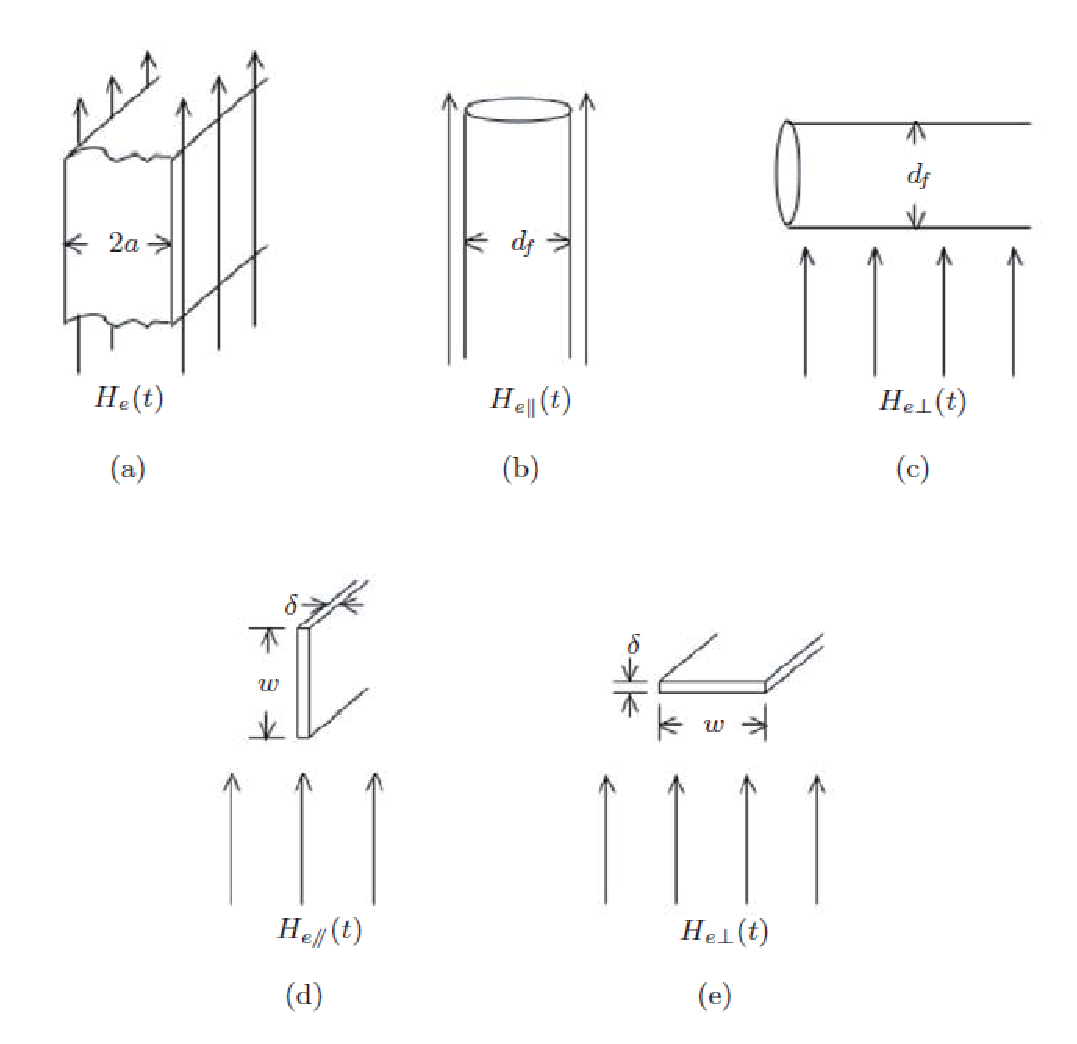
\includegraphics[scale=0.6]{chpt7/figs/fig7.1.eps}
	\caption{置于空间均匀时变磁场中的超导体。}
\end{figure}

\subsubsection*{时变磁场}
为了计算交流损耗,我们多数时候需要一个以磁场$H_m$或电流$I_m$最大幅值、频率$f$或周期$\tau_m$为变量的磁场或电流
的时间函数---如果频率多余一个,则$f$被视为主要频率。
“现实世界”的交流损耗非常复杂,即使采用程序也完全不可能精确的仿真问题,更别提交流损耗计算值的高精度了。
所以,建模为具有单一频率或周期的时间函数足够了,尤其是对粗略估算。

\subsubsection*{交流损耗的能量密度表}
交流损耗能量密度的闭式解析解总结如表7.3-7.9。表达式仅对图7.1给出的超导体配置和场方向有效;
对Bean板相关的表达式将在本章做推导。

\subsection{磁滞损耗}
如第二章所述,单位体积内的热耗散可以视为坡印廷矢量$\vec{S}$(方程2.20)流量。
积分形式下,忽略电能项,方程2.20成为:
\begin{equation}% 7.1
\int\left[-\int_{S}^{}\vec{E}\times\vec{H}\cdot d\vec{\ \mathcal{A}}\right]dt=\int_{\nu}^{}\left[\int\vec{E}\cdot\vec{J}dt+\frac{1}{2}\mu_oH^2+\mu_oH\int\vec{H}\cdot d\vec{M}\right]d\nu
\end{equation}
尽管Bean在他的第II类超导体磁场行为纯唯象(临界态模型)模型中使用了定义$\vec{B}=\mu_0(\vec{H}+\vec{M})$,
但如第五章所论及的,$B$是以超导体内磁场分布$H_s$下的“平均”磁感应强度$B_s$进行计算的,即$B_s(x)=\mu_0 H_s$。
因为Bean板仅在一个维度(x)上有限,$H_s(x)$和板内感应的超导电流密度$J_c$(Bean模型中,是依赖于场的)
仅在$x$方向变化。$J_c$是由电场$\vec{E}$建立起来的,后者是由$d\vec{B}(t)/dt$感应出来的。在Bean板中,
还可以写为均匀外磁场的时间变化率$\mu_0 d\vec{H_e}(t)/dt$。

\subsubsection*{Bean板的磁滞损耗}
所以,Bean的第II类超导体临界态模型中,$\vec{M}$是由$\vec{H_s}_x$表示的,后者又是由$\vec{J_c}$表示的。
相应的,宽度为$2a$的Bean板方程修改为:
\begin{equation}% 7.2
\int\left[-\int_{S}\vec{E}(x)\times\vec{H}_e\cdot d\vec{\ \mathcal{A}}\right]dt=\int_{0}^{2a}\left[\int\vec{E}(x)\cdot\vec{J}_c(x)dt+\frac{1}{2}\mu_oH_{s}^{2}(x)\right]dx
\end{equation}
式中,积分区间是$x=0$到$x=2a$(或者从$x=-a$到$x=a$)。
因为$\vec{J_c}(x)$是由$\vec{E}(x)$感应出的,所以它平行于$E$场。7.2中的$\int E(x)\cdot J_c(x)dt$表示的是
耗散,这个耗散被称为磁滞损耗。Bean板的磁滞损耗能量密度为:
\begin{equation}% 7.3a
e_{hy}=\frac{1}{2a}\int_{0}^{2a}\left[\int J_cE(x)dt\right]dx
\end{equation}
通过联立7.3和7.2,我们可以得到另一种表达式:
\begin{align*}% 7.3b
e_{hy}=\frac{1}{2a}\{\int\left[-\int_{S}\vec{E}(x)\times\vec{H}_e\cdot d\vec{\ \mathcal{A}}\right]dt-\frac{1}{2}\mu_oH\int_{0}^{2a}H_{s}^{2}(x)dx\} \tag{7.3'}
\end{align*}
方程7.3’表示板中的磁滞能量密度等于进入板的Poynting能量密度减去板中的磁能密度的总能量密度。

当外场$\vec{H}_e$经过一个完整周期,初始和终了磁场强度$\vec{H}_{e_i}$、$\vec{H}_{e_f}$
和磁化强度$\vec{M}(\vec{H}_{e_i})$和$\vec{M}(\vec{H}_{e_f})$都是相等的,$e_{hy}$于是还可以表示为:
\begin{equation}% 7.4a
e_{hy}=\mu_o\oint\vec{H}_ed\vec{M}_e(\vec{H}_e)
\end{equation}
从代数上看,上式还可以写为:
\begin{align*}% 7.4b
e_{hy}=-\mu_o\oint M(H_e)dH_e \tag{7.4'}
\end{align*}
在7.4’中,去掉了矢量符号。这是因为各矢量均仅有一个方向:$H_e$和$M$都是$y$向。

\subsubsection*{外磁场时间序列下的Bean板}
问题7.1-7.4和讨论7.1-7.2中,将研究Bean板置于外磁场在不同的时间序列下的磁滞能量密度。
情况1-6和情况1i-6i分别为板中无直流传输电流和有直流传输电流的情况,各情况由7.5定义。
\begin{equation}% 7.5
H_e(t)=0*(\ \mathrm{Virgin slab})\rightarrow H_m\rightarrow 0\rightarrow -H_m\rightarrow 0\rightarrow H_m\rightarrow 0\rightarrow -H_m\rightarrow 0
\end{equation}

简要描述方程7.5中给出的$H_e(t)$时间序列如下。
\begin{description}
	\item[情况1] $H_e(t)$从$0*$增加至$H_m$,其中$0*$表示板未经使用,即板中无超导电流密度$J_c$。
	\item[情况2] 这是情况1之后的场下降序列:$H_e(t)=H_m\rightarrow 0$。
	\item[情况3] 这是情况1和情况2的组合:$H_e(t)=0*\rightarrow H_m\rightarrow 0$。
	\item[情况4] 类似于情况1,但板已通过电流。
	\item[情况5] 类似情况2,但它紧随情况4:$H_e(t)=H_m\rightarrow 0$。
	\item[情况6] 开始于通过电流的的板,$H_e(t)$经过1个完整周期。
	\item[情况1i-6i] 除了一直同游直流传输电流,其他和对应的情况1-6一样。
\end{description}

情况1/2/4的$H_s(x)$图分别如图7.2-图7.4。没有传输电流时,板的磁场行为是关于中点$x=a$对称的;
因此,$H_s(x)$图仅给出$0\le x\le a$部分。情况1i-6i中的个别$H_s(t)$图后文给出。
\begin{figure}[htbp]
	\centering
	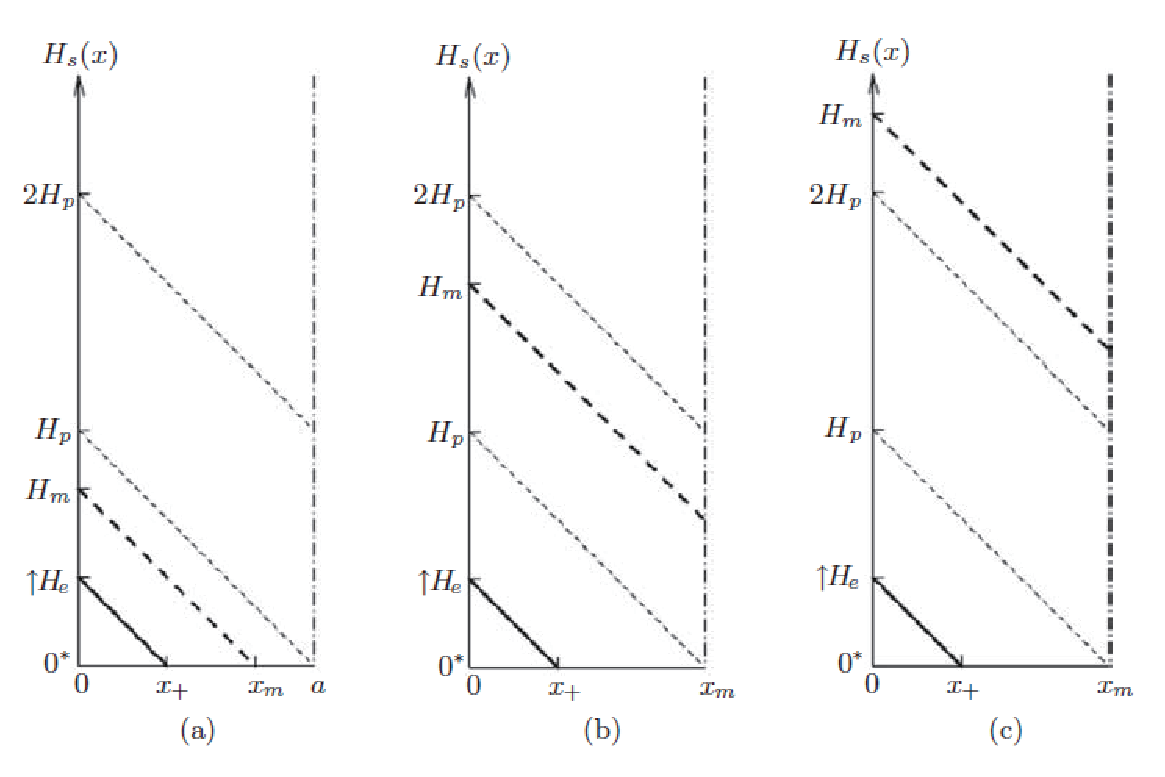
\includegraphics[scale=0.6]{chpt7/figs/fig7.2.eps}
	\caption{情况1的磁场特性。}
\end{figure}
\begin{figure}[htbp]
	\centering
	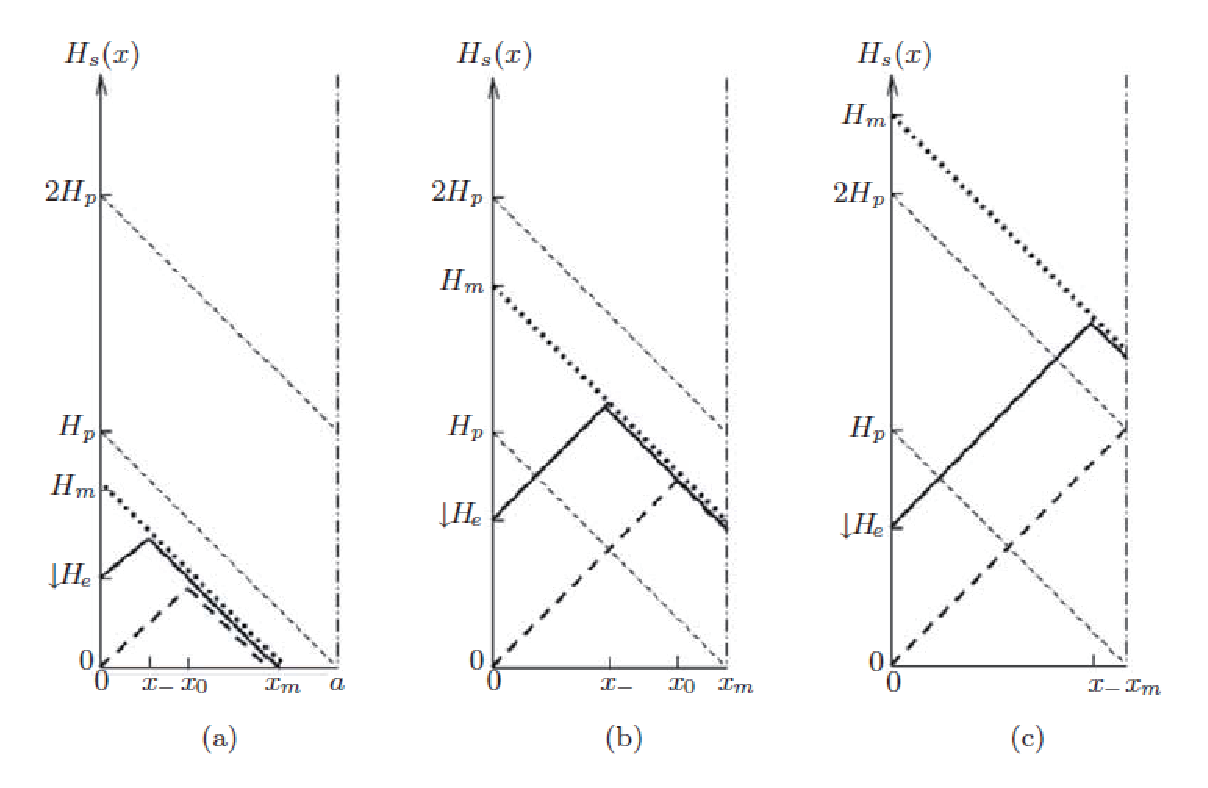
\includegraphics[scale=0.6]{chpt7/figs/fig7.3.eps}
	\caption{情况2的磁场特性。}
\end{figure}
\begin{figure}[htbp]
	\centering
	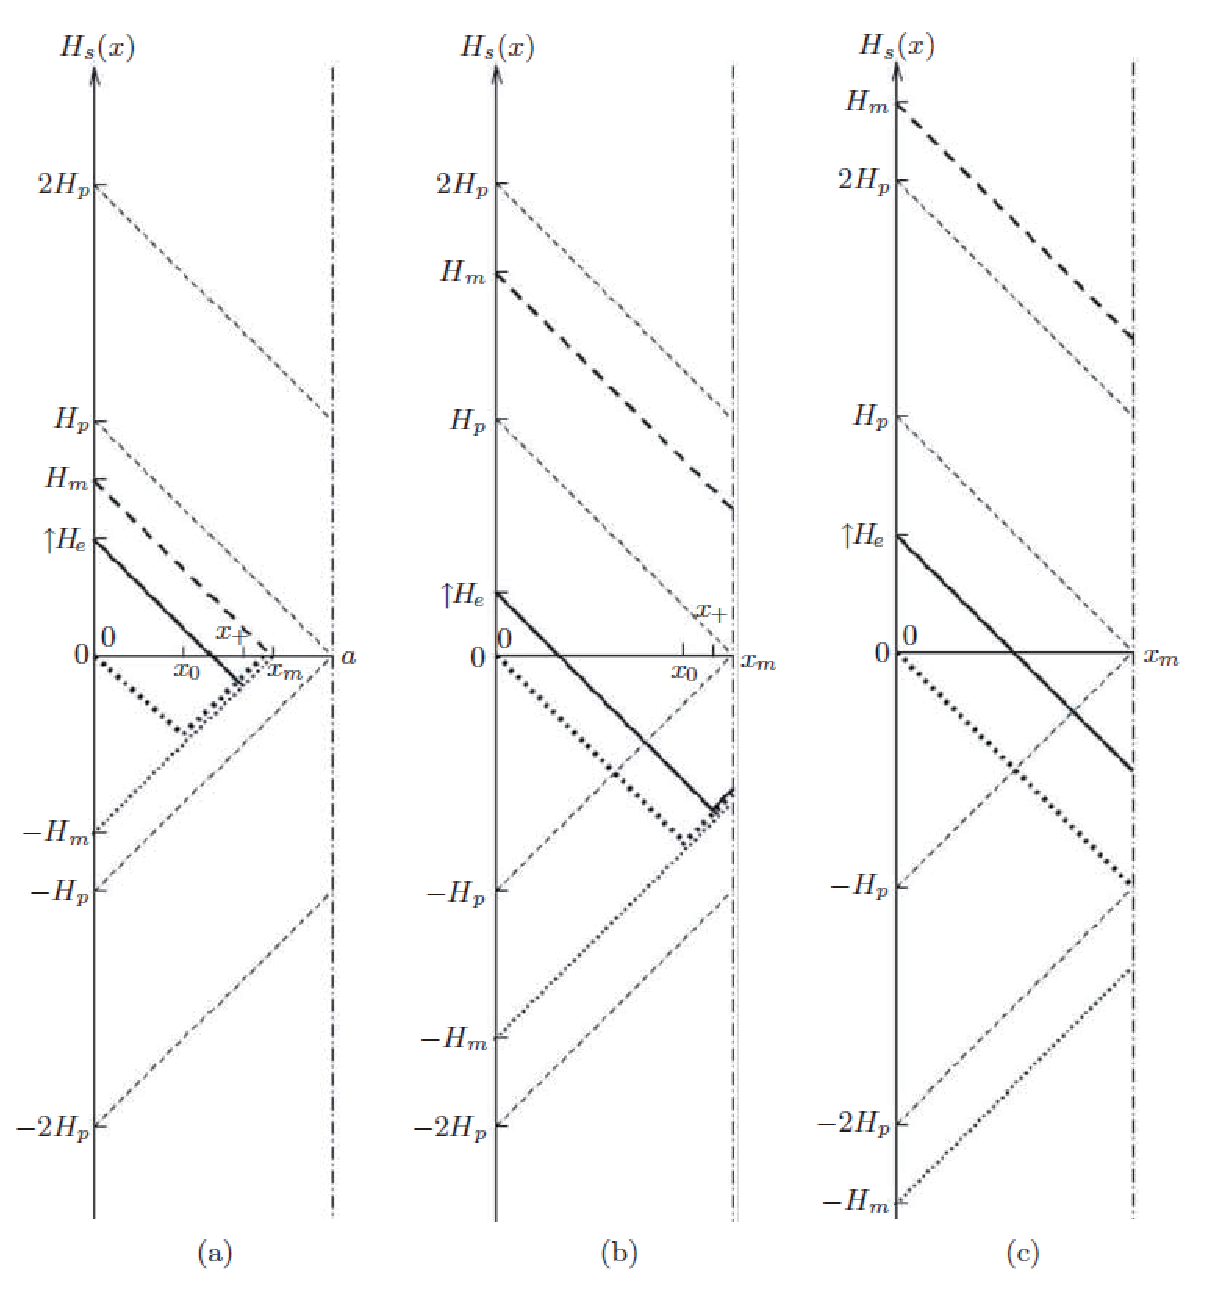
\includegraphics[scale=0.7]{chpt7/figs/fig7.4.eps}
	\caption{情况4的磁场特性。}
\end{figure}

\subsection{多丝复合物中的耦合损耗}
耦合损耗是多丝复合超导体中焦耳热的另一个形式,它来自时变外场在细丝之间感应出的耦合电流。
因为耦合电流通过金属基底金属,它随时间衰减。出于简单考虑,我们采用带有一个简单耦合时间常数$\tau_{cp}$
的指数模型。显然,$\tau_{cp}$越大,耦合电流在基底金属中流通的时间越长,造成的耦合能量损耗密度$e_{cp}$
越大。$\tau_{cp}$是耦合电流路径中电感$L$和电阻$R$的比值;$L/R$随着绕节距长度$\ell_p$的紧凑性增加而减小,
随基底金属电阻率增加而减少。图7.5给出了两根丝复合导体的示意图。多丝导体的复杂几何(比如换位丝就是复杂性的一个来源)
让基于Bean板的分析模型几乎不可能。
\begin{figure}[htbp]
	\centering
	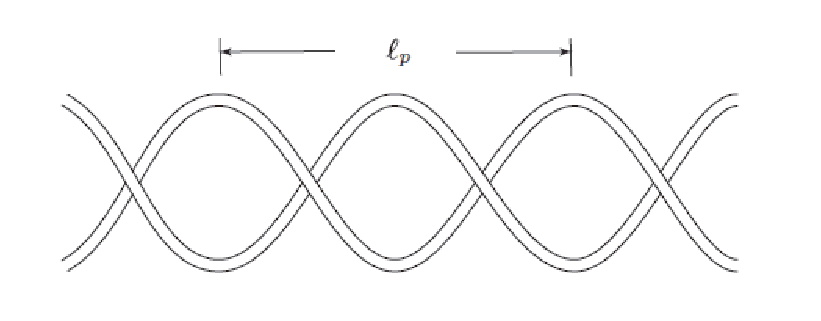
\includegraphics[scale=0.6]{chpt7/figs/fig7.5.eps}
	\caption{两根丝复合导体的示意图,使用方程7.6定义节距$\ell_p$。}
\end{figure}

\subsubsection*{耦合时间常数}
$e_{cp}$的关键参数是耦合时间常数$\tau_{cp}$。
它定义了多丝导体置于外时变场而感应出的丝间耦合电流的衰减时间常数。
实际中,电流衰减函数包括很多时间常数,不仅是主要的这一个。不过在实验中,
仅能确定主要的这一个,它被用于多数唯象方法中,$\tau_{cp}$定义为:
\begin{equation}% 7.6
\tau_{cp}=\frac{\mu_o\ell_{p}^{2}}{8\pi\rho_{ef}}
\end{equation}
式中,$\ell_p$是超导丝的节距,$\rho_{ef}$是丝间电流用到的有效基底电阻率。
如前所述,因为时间常数越长,能量耗散越大。故$\tau_{cp}$越大,$e_{cp}$越大。
正如Wilson指出[1.27]的,$e_{cp}$可以视为在复合导体内总磁能密度$\mu_0 H_m^2/2$的一部分,
当$\tau_{cp}\rightarrow 0$时有$e_{cp}\rightarrow 0$。
如前所述,有用的$e_{cp}$公式在表7.8给出;它包括了多丝线在四种外部磁场函数下的$e_{cp}$:1)
正弦;2)指数;3)三角波;4)梯形波。这些汉书的关键时间参数定义在图7.18中。

\subsubsection*{有效基底电阻}
我们将简要讨论方程7.5中出现的电阻率$\rho_{ef}$。它代表垂直于丝导体轴向的电流的基底有效电阻率。
Carr提出了两个模型[7.18]:
\begin{subequations}
	\begin{align}
	\rho_{ef0}&=\frac{1-\lambda_f}{1+\lambda_f}\rho_m\\
	\rho_{ef\infty}&=\frac{1+\lambda_f}{1-\lambda_f}\rho_m
	\end{align}
\end{subequations}
式中,$\lambda_f$是超导细丝在复合导体中的体积分数,$\rho_m$是基底的电阻率。

方程7.7a和7.7b基于图7.6中的两个极限电流分布:(a)中细丝表面的接触电阻是0,电流被拉入细丝中,令电路通路
的视在截面和距离分别变大和变小,故得到7.7a;(b)中恰好相反。
两个表达式都没有经受严格分析和试验的检验。实践中,方程7.7a和7.7b分别用于$\mathrm{Nb_3Sn}$和NbTi超导体的计算。

\subsection{涡流损耗}
涡流损耗的基本问题已在问题2.7中研究了。圆线(图7.1b和7.1c)和带材(图7.1d和7.1e)低频极限下的能量密度$e_{ed}$公式,总结如表7.9。
\begin{figure}[htbp]
	\centering
	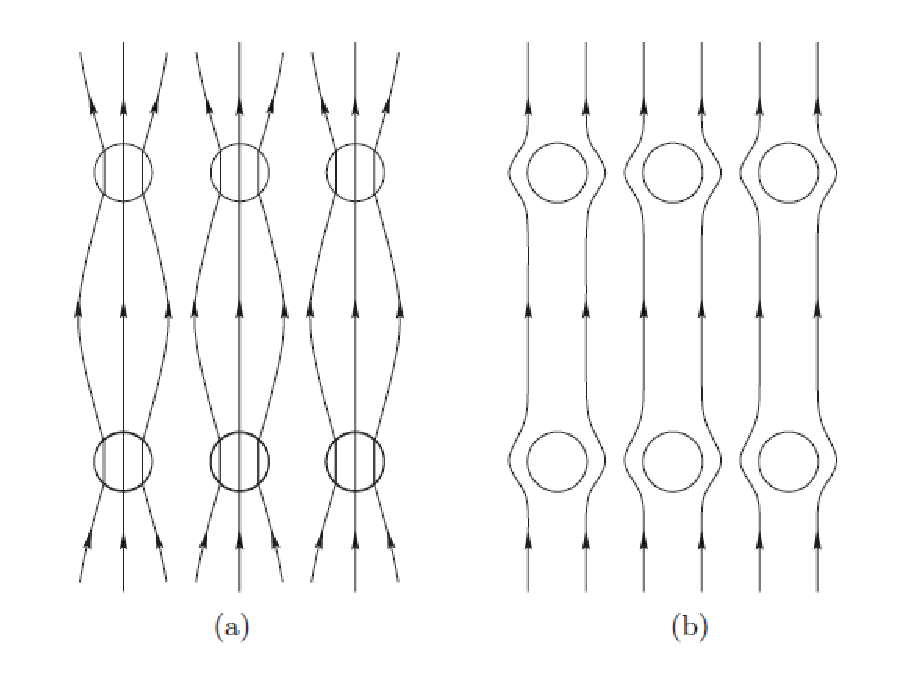
\includegraphics[scale=0.6]{chpt7/figs/fig7.6.eps}
	\caption{多丝超导体中垂直于导体轴的电流分布。}
\end{figure}

\section{其他损耗}
还有两个其他耗散源:1) 分段--或接头---电阻;和2) 机械扰动。
对于干式磁体的驱动模式,无论LTS还是HTS,必须将接头电阻处产生的损耗降至最低,原因很明显---它直接增加了制冷机的热负荷。
显然,这对持续运行模式的磁体不是问题---该模式要求接头近似为零,在$\mathrm{p\Omega}$数量级。
机械扰动---绕组内发生的导体运动或环氧浸渍绕组的环氧开裂---仅对“绝热”LTS磁铁重要;
对于冷却良好的LTS,最大的耗散源是复合超导体本身的焦耳热,机械扰动可以完全忽略。
处于一个不同的原因,如第6章所述,高HTS磁体,不论冷却良好或“绝热”,是不受这些机械扰动的影响的。
\subsection{接头电阻}
只有在以下情况下,电阻型接头才会成为设计问题:1)必须限制在受限空间内或遵从特定配置;
2)位于绕组内部较深的地方,那里的冷却有限或为零;3)必须承受较大的力;4)接头太多,其累积耗散会对系统的制冷负担加重。
5)不与制冷剂直接接触,如在低温冷却磁体中那样。

大致来讲,有两种类型接头:搭接接头和对接接头。
在大多数应用中,搭接接头比对接接头更好,原因有三个:1)比对接接头更容易制作;
2)通过简单增加搭接长度可以任意降低接头电阻;3)通常比对接接头更容易满足强度要求。
这里,我们讨论搭接拼接。

\subsubsection*{搭接电阻(接头)}
如图7.7所示,“握手式”搭接接头是最广泛使用的接头设计;它甚至非常适合在绕组内使用。
导线A和导线B之间的接头以搭接长度$\ell_{sp}$、宽度$a$和厚度$\delta_{sd}$经焊接而电气连接。
焊料电阻率为$\rho_{sd}$的焊料层电阻$R_{sd}$可由下式给出:
\begin{equation}% 7.8
R_{sd}=\frac{\rho_{sd}\delta_{sd}}{a\ell_{sp}}
\end{equation}
通常,$a$等于搭接导体的宽度。
\begin{figure}[htbp]
	\centering
	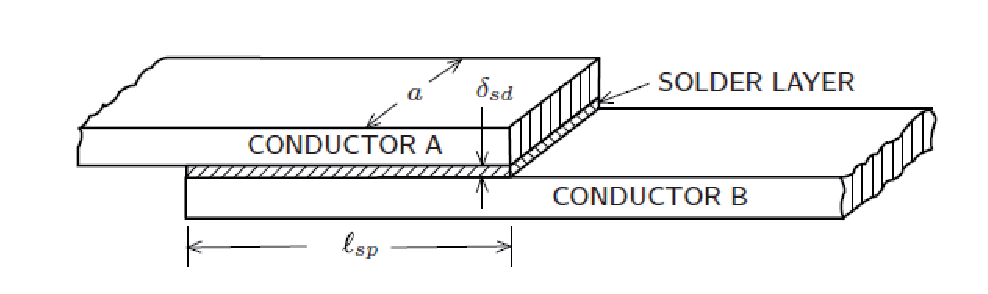
\includegraphics[scale=0.6]{chpt7/figs/fig7.7.eps}
	\caption{“握手式”搭接接头。}
\end{figure}

\subsubsection*{接触电阻}
接头电阻$R_{sp}$是以下三个部分之和:
\begin{subequations}
	\begin{align}
R_{sp}&=R_{cA}+R_{sd}+R_{cB} \\
&=\frac{R_{ct}}{A_{ct}}
	\end{align}
\end{subequations}
式中,$R_{cA}$是导体A和焊接层之间的接触电阻,$R_{cB}$是导体B和焊接层之间的接触电阻。
$R_{ct}$是接触电阻,单位为$[\Omega m^2]$,$A_{ct}=a\ell_{sp}$是接触面积。
如果焊接剂“湿润”了各导体的表面,则假设$R_{cA}\simeq R_{cB}\simeq 0$是合理的,至少假设
$R_{cA}\simeq R_{cB}\ll R_{sd}$是合理的:
\begin{align*}% 7.9c
R_{sp}=\frac{R_{ct}}{A_{ct}}\simeq R_{sd} \tag{7.9c}
\end{align*}
通过令$\ell_{sp}$足够长,$R_{sp}$可以任意小。联立7.8和7.9c,有:
\begin{align}% 7.10
R_{ct}\simeq\rho_{sd}\delta_{sd}
\end{align}
因此,我们可以选择低电阻率焊料来实现“小”$R_{ct}$。同样重要的是,最小化$\delta_{sd}$,一定不要超过10-50 $\mu$m。
实际上,如果使用“超导”焊料,则$R_{ct}$为零,只要这种接头工作在低场区,并提供了足够电流传输面积$a\ell_{sp}$。
利用超导焊料,可以制作$\mathrm{p\Omega}$数量级的超导接头。
这种接头必须工作于低场($\le 1$ T)和深冷($\le 9$ K)环境中,要有足够的接触面积以便在接头承载工作电流时保持焊料超导。

表7.1列出了所选锡铅焊料的$R_{ct}$值。$R_{ct}$是磁场依赖的,随B线性增加。
在一些数据中,在0和1T之间观察到了非线性。这些数据仅作为一般指南给出。
在涉及大型磁体的项目中,接头电阻是一个重要的设计问题,明智的做法是根据实测值确定。


表7.1.。。。。。。。。。。。。。。。。。。

表7.2.。。。。。。。。。。。。。。。。。。

表7.2列出了Fujishiro[7.21]给出In和六种常用合金焊料的零场电阻率 vs. 温度的数据。
其中,$T_{sl}$和$T_{lq}$分别是固相线和液相线温度。(这些温度的差异越小,焊接越容易;当$T_{sl} = T_{lq}$时,
合金具有明确的熔点。)如表中所示,这些常见的焊料合金可在4.2 K以上超导;$T_c$是零场临界温度[4.41,4.42,7.20]。

\subsubsection*{机械接触开关}
对于某些应用,使用机械接触开关比使用热激活持续电流开关(persistent current switch, PCS)更有利。
铜或涂铟铜表面之间的机械接触电阻虽然很小,但在4.2 K时也不超导[7.22]。
最近,Sawa等研究了利用工作在77 K的HTS块盘之间的机械接触构建机械接触开关[7.23,7.24]。
尽管在77 K下明显不超导,但如果在低于10 K的温度下运行,且用涂有超导焊料的HTS块材盘,
则可以实现超导机械接触开关的盘到盘超导接触。

\subsection{机械扰动}
直到1970年代,多数磁体(当然全都是LTS的)都是根据Stekly稳定性标准建造的。这些磁体是很好(局域的)冷却
且低$\lambda J_{op}$的磁体,从而机械扰动不是大问题---
绕组设计主要处理大焦耳热耗散。
只有当运行在磁体在高$\lambda J_{op}$成为必须,如在高能物理粒子加速器的偶极和四极磁体以及“商业上可行的”NMR和MRI磁体中,
机械扰动才成为关键的设计问题。
增强$\lambda J_{op}$的一个显而易见的方法是去掉制冷工质占用的空间,并用产生场的导体或承载材料取代至---
催生了绝热LTS磁体。这些磁铁很容易在很小的$g_d$水平下失超。
通过使用下面描述的声发射(AE)技术,1980年代中期明确了机械扰动事件(主要是导体运动或浸渍填充材料的破裂)
几乎是这些绝热LTS磁体每次“过早失超”事件的原因。


没有冷却使绝热磁体过早地失超,有时电流远低于其预期工作电流时就失超了。
幸运的是,这些机械事件通常遵循声发射中已知的那些“Kaiser效应”。
它描述了在一系列循环负荷过程中观察到的机械行为。过程中,机械扰动如导体运动和环氧树脂破裂仅在引起事件的负荷超过任何先前加载顺序中达到的最大水平时,才出现。
因此,易过早失超的绝热磁体通过“锻炼”以逐渐改善其性能,使其最终达到预期的工作电流。
显然,设计绝热磁体的目的是让它在第一次尝试时就达到工作电流;
如此显著的成果只是偶尔才能遇到,例如750 MHz(17.6 T)NMR磁体[7.25]。

如前所述,自1980年代中期以来,已经引入了针对这些机械扰动的补救措施。
如今,大多数绝热LTS磁体大部分时间都摆脱了此类威胁事件。
下面简要描述导体运动和填充材料的破裂以及针对这些机械扰动的补救措施。

\subsubsection*{导体运动和补救}
即使导体以完美有序方式“密”绕,如紧密堆积的六边形,绕组仍然足够松,导体在洛伦兹力的作用下不足以摩擦力抵抗移动。
我们可以估计在典型的运行条件下绝热地驱动单位导体体积到正常态所需的摩擦位移的量,并且表明这种位移确实是可能的。
比如,一个导体$r$ = 0.2 m,置于5 T的z向场$B_z$中,在$\theta$向上载流密度(在导体横截面上)
$J_\theta= 200\times 10^6\ \mathrm{A/m^2}$,
受到$r$向洛伦兹力密度$f_{L_r} =J_\theta B_z=2\times 10^8\ \mathrm{N/m^3}$。
假设导体在$f_{L_r}$下反向滑移距离$\Delta r_f$;
在单位导体体积上的这种运动的摩擦能量密度$e_f$可由下式给出:
\begin{equation}% 7.11
e_f=\mu_ff_{L_r}\Delta r_f
\end{equation}
式中,$\mu_f$是摩擦系数。代入$\mu_f=0.3$和$e_f=1300\ \mathrm{J/m^3}$(铜在4.2 K和5.2 K之间的焓差),以及
$f_{L_r}=2\times 10^8\ \mathrm{N/m^3}$,在7.11中解出$\Delta r_f$:
\begin{align*}% page411最后一个
\Delta r_f=\frac{e_f}{\mu_ff_{L_r}}=\frac{(1300\ \mathrm{J/m^3})}{(0.3)(2\times 10^8\ \mathrm{N/m^3})}\simeq 20\times 10^{-6}\ \mathrm{m}=20\ \mathrm{\mu m}
\end{align*}

即使在紧密有序的绕组中也几乎不可能避免滑动这么小的距离。
如在一系列实验[7.26-7.31]中观察到的,小至$\sim 10\ \mathrm{\mu m}$的滑动足以引发失超。

关于微小滑移的补救措施是用绝缘材料浸渍绕组,绝缘材料通常以流体填充空隙空间,随后转变为成固体。
浸渍将整个绕组变为成整体结构件。现在,几乎每个绝热LTS磁体都浸渍有石蜡、环氧树脂等填充材料,有些还掺杂其他粉末以获得“强化”它和/或提高其导热性。
 
\subsubsection*{填充材料破裂和补救}
尽管在浸渍绕组中可能不存在导体运动,但仍存在两个问题。
首先,在洛伦兹力作用下,整个绕组体---螺线管磁体---有变成桶形的趋势。
除非绕组牢固地固定在线圈骨架上以防止这种桶形变形,否则在绕组和骨架之间会发生界面运动;
这种运动产生热,可能导致过早失超。
借助于粘合到绕组内表面的低导热性薄片,可以解耦导体与这种摩擦加热[7.32]。
其次,如果绕组牢固地贴合在骨架上,则绕组中产生大应力,并且浸渍剂可能破裂,成为另一个热扰动源。

在浸渍绕组中,两种方法可以防止由填充材料破裂引起的过早失超:1)最小化由断裂引起的能量;
2)完全消除破裂事件。尽管已有在低温下测量破裂引起的能量的尝试[7.33,7.34],但是我们对破裂机制的理解还不够,
所以这个方法暂时无用。

在消除破裂事件的第二种补救措施方面取得了很大进展。发展出的技术包括:1)在缠绕过程中对导体进行分级预应力[7.35];
2)允许绕组部分相对骨架“浮动”[7.35,7.36]。
 Maeda已将这种浮动绕组概念推向极限,并通过“无骨架”螺线管成功实现了性能[7.37]。
 现在,多数浸渍绕组都是相对骨架“浮动”的,使运行在4.2 K或更低温度的绝热LTS实达到其运行电流。
 可能第一次尝试不行,但通常在经过几次“锻炼”失超后可以实现。


\section{声发射技术}
\subsection{机械事件探测——LTS磁体}
通常,当超导磁体受到(或卸掉)磁应力时,时变应变在超导磁体中产生AE信号。
本技术开始于1970年代后期[7.38-7.40],成形于1980年代:两个影响高性能LTS磁体的主要的机械事件---
导体运动和环氧树脂破裂---可以通过AE技术[7.41-7.54]检测出。
在超导磁体中最有效地使用AE是Brechna和Turowski在1978年首次报道的AE/电压技术[7.40]。
因为突然的导体运动事件产生AE信号---信号在绕组内以2-5 km/s的典型速度传播---
同时在磁体端子上诱导出电压脉冲,在失超时同时检测到AE和电压信号表明它是由导体运动引起的---
在存在磁场的情况下,一小段导体的位置突然移动,由法拉第定律知道,将产生跨越绕组端子的电压脉冲。 
AE技术还可用于证明伴随AE信号而非电压尖峰的失超最可能由其他机械事件(例如环氧树脂裂缝)引起。
图7.8显示了Nb3Sn线圈的过早失超;在电阻性失超电压之前出现的电压脉冲的开始伴随出现的AE信号
强烈表明这种过早失超是由导体运动触发的[7.54]。

\subsection{应用于HTS磁体}
除了磁力外,超导磁体中另一个重要的时变应变源是时变的非均匀温度分布。
事实上,当磁铁冷却(或加热)时,会产生AE信号。
实际上,在LTS磁体中观察到主要来源为随时间变化的非均匀温度分布[7.55,7.55]产生的AE信号。
图7.9显示了达到其临界电的偶极磁体上记录的一个波形图流[7.57]。
因为失超是“自然的”,所以在失超开始时没有触发AE信号。
然而,如SENSOR 1所记录的,在失超开始后约5ms出现AE信号。
AE信号很可能是由失超产生的不均匀温度分布引起的,虽然“自然”触发,但是它位于高场区域。

\begin{figure}[htbp]
	\centering
	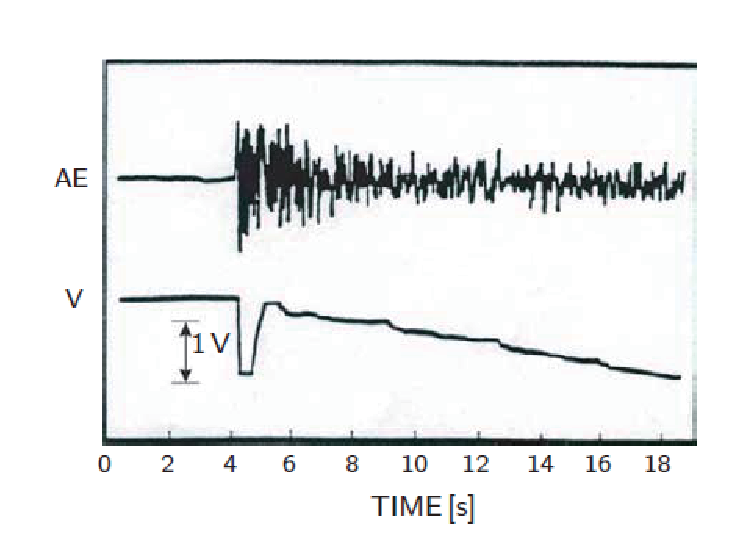
\includegraphics[scale=0.6]{chpt7/figs/fig7.8.eps}
	\caption{Nb3Sn线圈过早失超时的AE和电压信号。}
\end{figure}

AE信号可以作为电压信号的补充一同用于HTS磁体中过热开始的检测,
特别是因为HTS的电阻电压由于其低指数而不会像LTS那样急剧上升。
Wozny等人记录了YBCO大量块材样品中超导---正常转变中因温度升高产生的AE信号[7.58];
Arai在用Bi2223缠绕的实验饼式线圈中检测到了热诱导的AE信号[7.59]。
进一步的让AE信号成为电压信号有益补充以保护HTS磁体的努力还在进行中[7.60]。

\begin{figure}[htbp]
	\centering
	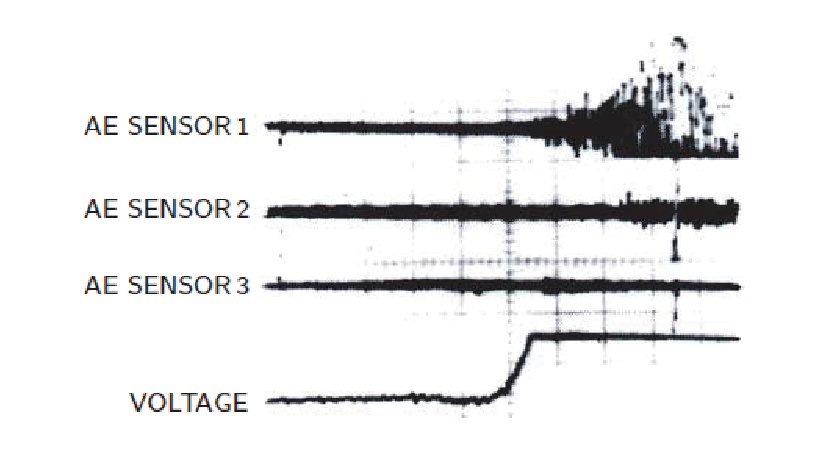
\includegraphics[scale=0.6]{chpt7/figs/fig7.9.eps}
	\caption{一个在其临界电流的超导磁体“自然”失超时的AE信号和电压的波形图(时间刻度: 2ms/div)。}
\end{figure}

\section{专题}
\subsection{问题7.1:磁滞能量密度——在“小”磁场时间序列的“无染”Bean板}
考虑一个宽$2a$的“无染”Bean板,置于情况1所述的增长磁场序列中,$H_e=0*\rightarrow H_m\le H_p$(“小”磁场),
其中$0*$表示Bean板是“无染”的,$H_p=J_c a$。
而后,将之置于如情况2所述的降低磁场序列中,$H_e=H_m\rightarrow 0$。
情况3的磁场序列就是情况1后紧随情况2。
情况1的$-M(H_e)$如方程5.5,情况2相应的被修正为方程5.7:
\begin{align*}% 5.5
-M(H_e)=H_e-\frac{H_{e}^{2}}{2H_p} \quad (H_e=0*\rightarrow H_m\leq H_p) \tag{5.5}
\end{align*}
\begin{equation}% 7.12
-M(H_e)=H_e+\frac{H_{e}^{2}-2H_mH_e-H_{m}^{2}}{4H_p}   \quad   (H_e=H_m\rightarrow 0)
\end{equation}

图7.10给出了上面两个方程的$-M(H_e)$。

a) 对半板($0\le x\le a$)应用7.13,证明情况1$H_e=0*\rightarrow H_m$下的$e_{hy}$为:
\begin{align*}% 7.13a
e_{hy}=\frac{\mu_oH_{m}^{3}}{6H_p}  \quad      (0\leq H_m\leq H_p) \tag{7.13b}
\end{align*}

b) 类似的,对半板($0\le x\le a$)应用7.13,证明情况2$H_e=H_m\rightarrow 0$下的$e_{hy}$为:
\begin{align}% 7.14a
e_{hy}=\frac{\mu_oH_{m}^{3}}{24H_p}  \quad     (0\leq H_m\leq H_p)
\end{align}

c) 使用7.3b,证明情况3$H_e=0*\rightarrow H_m\rightarrow 0$下的$e_{hy}$显然为方程7.13和7.14之和:
\begin{equation}% 7.15a
e_{hy}=\frac{5\mu_oH_{m}^{3}}{24H_p}      (0\leq H_m\leq H_p)
\end{equation}
\begin{figure}[htbp]
	\centering
	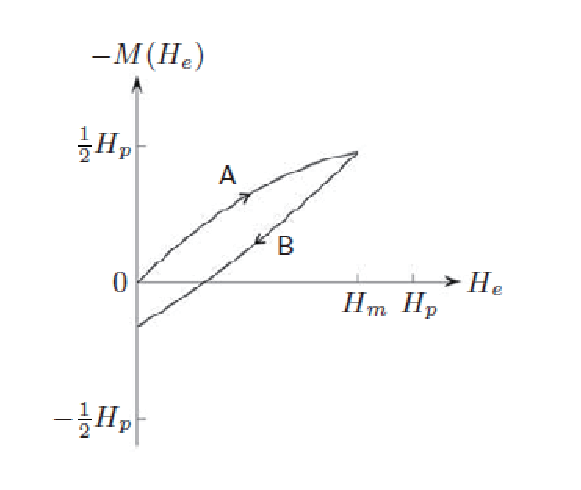
\includegraphics[scale=0.7]{chpt7/figs/fig7.10.eps}
	\caption{“小”磁场激励($H_m\le H_p$)下的$-M(H_e)$。序列A开始于原点,即“无染”Bean板。}
\end{figure}

\subsubsection{问题7.1之解}
a) 在增长磁场序列$H_e=0*\rightarrow H_m$下,首先找到当外场增加过程中的$E_z(x)dt$的表达式。
板内的$H_s(x)$如图7.2a中的实线所示。板内的$x=0$和$x=x_+(=H_e/J_c)$之间,因磁场变化$dH_e/dt$引起的$E_z(x)$
可以表示为:
\begin{align*}% page416 1
E_z(x)=\mu_o\frac{dH_e}{dt}(x_+-x) \tag{S1.1a}
\end{align*}
\begin{align*}% page416 2
E_z(x)dt=\mu_o(x_+-x)dH_e \tag{S1.1b}
\end{align*}
对前半板应用方程7.3a和S1.1b,有:
\begin{align*}% page416 3 and 4
e_{hy}=\frac{1}{a}\int_{0}^{a}\left[\int J_cE(x)dt\right]dx \tag{S1.2a}
\end{align*}
\begin{align*}
=\frac{\mu_oF_c}{a}\int_{0}^{H_m}\left[\int_{0}^{x_+(x_+-x)dx}\right]dH_e \tag{S1.2b}
\end{align*}
在方程S1.2b中,因为$x_+$依赖于$H_e$,积分顺序和S1.2a相反。方程S1.2b成为:
\begin{align*}% page416 5 and 6
e_{hy}=\frac{\mu_oJ_c}{a}\int_{0}^{H_m}\left(x_{+}^{2}-\frac{x_{+}^{2}}{2}\right)dH_e  \tag{S1.2c}
\end{align*}
\begin{align*}
=\frac{\mu_oJ_c}{a}\int_{0}^{H_m}\frac{H_{e}^{2}}{2J_{c}^{2}}dH_e=\frac{\mu_oH_{m}^{3}}{6aJ_c} \tag{S1.2d}
\end{align*}
\begin{equation}% 7.13a
e_{hy}=\frac{\mu_oH_{m}^{3}}{6H_p} \quad   (H_m\leq H_p) \tag{7.13a}
\end{equation}
$e_{hy}\propto H_m^3$;也即,在“小”磁场激励下,$e_{hy}$以$H_m$的三次方增加;这已被很多实验所验证。

b) 在降低的磁场序列$H_e=H_m\rightarrow 0$中,$E_z(x)$由下式给出:
\begin{align*}% page416 S1.3
E_z(x)dt=\mu_o(x-x_-)dH_e \tag{S1.3}
\end{align*}
式中,$x_-=(H_m-H_e)/2J_c$,如图7.3a所示。所以,$e_{hy}$为:
\begin{align*}% page416 S1.4
e_{hy}&=\frac{\mu_oJ_c}{a}\int_{H_m}^{0}\left[\int_{0}^{x_-}(x-x_-)dx\right]dH_e=\frac{\mu_oJ_c}{a}\int_{H_m}^{0}\left(\frac{x_{-}^{2}}{2}-x_{-}^{2}\right)dH_e \\\tag{S1.4}
&=\frac{\mu_oJ_c}{a}\int_{H_m}^{0}\frac{(H_m-H_e)^2}{8J_{c}^{2}}dH_e=\frac{\mu_oH_{m}^{3}}{24aJ_c}
\end{align*}
\begin{align*}% 7.14a
e_{hy}=\frac{\mu_oH_{m}^{3}}{24H_p}  \quad     (0\leq H_m\leq H_p) \tag{7.14a}
\end{align*}
在降低的磁场序列中,$e_{hy}$是增长磁场序列的$1/4$。
根据图7.2a和7.3a,这是因为情况1中$E_z$是在$x=0$和$x_m=H_m/J_c$之间感应出的,而在情况2中,
是在$x=0$和$x_0=H_m/2J_c$之间感应出的;此时仍有$e_{hy}\propto H_m^3$。

c) 板中的E场,由它的下标$z$可知,是指向$z$向的。特别的,当$H_e(t)$指向$+y$向时,E指向$-z$向。
这样,在板表面($x=0$),坡印廷矢量$\vec{S}$指向$+x$向,因为在第一个序列$H_e=0*\rightarrow H_m$下,
能量从外部空间进入板内,被储存和耗散。在第一个序列中,$E_z(0)$由S1.1b给出($x_+=H_e/J_c$):
\begin{align*}% page417 S1.5a
E_z(0)=\mu_o\frac{H_e}{J_c}\left(\frac{dH_e}{dt}\right) \tag{S1.5a}
\end{align*}
方程7.3b的右侧第一项是情况1的坡印廷能量密度$e_{py1}$,可以写成:
\begin{align*}% page417 S1.6a两个
e_{py1}\equiv\frac{1}{a}\int\left[-\int_{S}\vec{E}(x)\times\vec{H}_e\cdot d\vec{\ \mathcal{A}}\right]dt=\frac{\mu_o}{aJ_c}\int_{0}^{H_m}H_{e}^{2}dH_e\\
e_{py1}=\frac{\mu_oH_{m}^{3}}{3H_p} \tag{S1.6a}
\end{align*}
情况2中,$E_z(0)$由方程S1.3给出,此时$x_-=(H_m-H_e)/2J_c$:
\begin{align*}% page417 S1.5b
E_z(0)=-\mu_o\left(\frac{H_m-H_e}{2J_c}\right)\frac{dH_e}{dt} \tag{S1.5b}
\end{align*}
于是,情况2的坡印廷能量密度$e_{py2}$为:
\begin{align*}% page417 S1.6b两个
e_{py2}=\frac{\mu_o}{2aJ_c}\int_{H_m}^{0}(H_m-H_e)H_edH_e\\
e_{py2}=-\frac{\mu_oH_{m}^{3}}{12H_p} \tag{S1.6b}
\end{align*}
方程S1.6b中的$-$号表示$e_{py2}$是流回源的。在整个序列结束$H_e=0*\rightarrow H_m\rightarrow 0$(情况3)的时候,
有方程7.12可知,$-M(0)=-H_m^2/4H_p$:
板通过$H_s(x)$储存的磁场(或磁化)能量密度$e_{m_f}$为($x_0=H_m/2J_c$):
\begin{align*}% page417 S1.7a
H_s(x)=J_cx  \quad      (0\leq x\leq x_0) \tag{S1.7a}
\end{align*}
\begin{align*}% page417 S1.7b
H_s(x)=H_m-J_cx  \quad  (x_0\leq x\leq H_m/J_c) \tag{S1.7b}
\end{align*}
使用方程S1.7a和S1.7b,我们可以计算$e_{m_f}$:
\begin{align*}% page417 S1.8
e_{m_f}=\frac{\mu_o}{2a}\int_{0}^{a}H_{s}^{2}(x)dx&=\frac{\mu_o}{2a}\left(2\times\int_{0}^{\frac{H_m}{2J_c}}J_{c}^{2}x^2dx\right)\\
e_{m_f}&=\frac{\mu_oH_{m}^{3}}{24H_p} \tag{S1.8}
\end{align*}
联立7.3b/S1.6a/S1.6b/S1.8,我们得到情况3的$e_{hy}$:
\begin{align*}% 7.15a两个
e_{hy}&=e_{py1}+e_{py2}-e_{m_f} \\
&=\frac{\mu_oH_{m}^{3}}{3H_p}-\frac{\mu_oH_{m}^{3}}{12H_p}-\frac{\mu_oH_{m}^{3}}{24H_p}\\
e_{hy}&=\frac{5\mu_oH_{m}^{3}}{24H_p}   \quad    (0\leq H_m\leq H_p) \tag{7.15a}
\end{align*}

\textbf{能流}

这里我们检视一下在各磁场序列过程中从源到板的能流。每一个过程中,能量密度必须平衡:
\begin{align*}% page418 S1.9
e_{py}=e_{hy}+e_{m_f}-e_{m_i} \tag{S1.9}
\end{align*}
式中,$e_{m_f}$和$e_{m_i}$分别是板中终了和初始时的磁场能密。
本质上,S1.9和7.2是一样的。

在第一个序列中,$e_{py}=e_{py1}$(方程S1.6a),$e_{hy}$(方程7.13a),$e_{m_i}=0$(因为板处于“无染”态)和$e_{m_{f1}}$
可以由$H_s(x)=H_m-J_c x$计算:
\begin{align*}% page418 S1.10两个
e_{m_{f1}}&=\frac{\mu_o}{2a}\int_{0}^{a}H_{s}^{2}(x)dx \\
&=\frac{\mu_o}{2a}\left[\int_{0}^{\frac{H_m}{J_c}}(H_m-J_cx)^2dx\right]\\
e_{m_{f1}}&=\frac{\mu_oH_{m}^{3}}{6H_p} \tag{S1.10}
\end{align*}
将7.13a和S1.10代入S1.9的右侧,有:
\begin{align*}% page418 S1.11a
e_{py1}=\frac{\mu_oH_{m}^{3}}{6H_p}+\frac{\mu_oH_{m}^{3}}{6H_p}=\frac{\mu_oH_{m}^{3}}{3H_p} \tag{S1.11a}
\end{align*}
方程S1.11a中的$e_{py1}$和方程S1.6a中的是一致的,表明在第一个过程中能量密度流是平衡的。

我们还可以检视第二个过程$H_e=H_m\rightarrow 0$的能量平衡。这个过程中,S1.9方程右侧需要出现的能量密度是:
$e_{hy}$(方程7.14a),$e_{m_f}$(方程S1.8)和$e_{m_i}=e_{m_{f1}}$(方程S1.10):
\begin{align*}% page418 S1.11b
e_{py2}=\frac{\mu_oH_{m}^{3}}{24H_p}+\frac{\mu_oH_{m}^{3}}{24H_p}-\frac{\mu_oH_{m}^{3}}{6H_p}=\frac{\mu_oH_{m}^{3}}{12H_p} \tag{S1.11b}
\end{align*}
方程S1.11b中的$e_{py2}$等于方程S1.6b中的$e_{py2}$,表明在第二个过程中S1.9的能量平衡是成立的。
如前所述,$-$号表明在第二个过程中存在由板向源的净能量流:
这个能流密度加上磁滞能量流密度对应板中储存磁能的净减少量。


\subsection{问题7.2:磁滞能量密度——在“中”磁场时间序列的“无染”Bean板}
这里,我们研究在“中”磁场激励下的情况1-3,$H_p\le H_m\le2H_p=2J_c a$。
在增长磁场$H_e=0*\rightarrow H_m$序列中(情况1和3),$e_{hy}$在$H_m\ge H_p$时与$H_m$无关
---当然,Bean临界态模型中的$J_c$也与磁场无关。增长磁场和降低磁场序列中的$−M(H_e)$函数为:

\begin{align*}% 5.5和5.6
-M(H_e)=H_e-\frac{H_{e}^{2}}{2H_p}    \quad  (H_e=0*\rightarrow H_p) \tag{5.5}
\end{align*}
\begin{align*}
-M(H_e)=\frac{1}{2}H_p      \quad  (H_e=H_p\rightarrow H_m) \tag{5.6}
\end{align*}
\begin{align*}
-M(H_e)=\frac{1}{2}H_p-(H_m-H_e)+\frac{(H_m-H_e)^2}{4H_p} \quad   (H_e=H_m\rightarrow 0)\tag{5.7a}
\end{align*}

图7.11给出了方程5.5/5.6和5.7a给出的$−M(H_e)$。

a) 对半板($0\le x\le a$)应用方程7.3a,证明情况1下的$e_{hy}$为:
\begin{align*}% 7.13b
e_{hy}=\frac{1}{2}\mu_oH_pH_m\left(1-\frac{2H_p}{3H_m}\right)\quad   (H_p\leq H_m\leq 2H_p)\tag{7.13b}
\end{align*}

b) 对情况2,解释为什么$e_{hy}$仍可以由7.14a给出。

c) 使用7.3b,证明情况3下的$e_{hy}$是7.13b和7.14a之和,可由下式给出:
\begin{align*}% 7.15b
e_{hy}=\frac{1}{2}\mu_oH_pH_m\left[1-\frac{2H_p}{3H_m}+\frac{1}{12}\left(\frac{H_m}{H_p}\right)^2\right]     \quad (H_p\leq H_m \leq 2H_p) \tag{7.15b}
\end{align*}

d) 证明在$H_m=H_p$时,方程7.15a和7.15b给出同样的$e_{hy}$。

\begin{figure}[htbp]
	\centering
	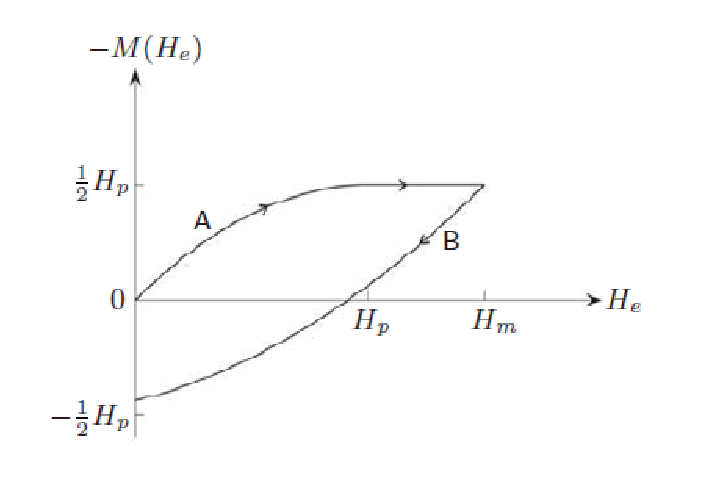
\includegraphics[scale=0.7]{chpt7/figs/fig7.11.eps}
	\caption{“中”磁场激励($H_m\le H_p$)下的$-M(H_e)$。$H_p\le H_m\le 2H_p=2J_c a$。}
\end{figure}

\subsubsection{问题7.2之解}
a) 情况1的前半部分中,$H_e=0*\rightarrow H_p$序列下,我们通过向方程7.13a中代入$H_m=H_p$获得
磁滞能量密度$e_{hy1'}$:
\begin{align*}% page420 S2.1
e_{hy1^\prime}=\frac{1}{6}\mu_oH_{p}^{2}  \quad     (H_e=0\rightarrow H_p) \tag{S2.1}
\end{align*}
这里,对情况1的后半部分,$H_e=H_p\rightarrow H_m$序列下,整个板的场参数(考虑对称性,我们仅取其中的一半
,从$x=0$到$x=a$)如图7.2b的虚线所示。$dH_e/dt$感应出的$E_z(x)$为:
\begin{align*}% page420 S2.2
E_z(x)=\mu_o\frac{dH_e}{dt}(a-x) \tag{S2.2}
\end{align*}
将方程7.3a和S2.2应用到半板上,有:
\begin{align*}% page420 S2.3a和2.3b
e_{hy1''}&=\frac{1}{a}\int_{0}^{a}\left[\int J_cE(x)dt\right]dx=\frac{\mu_oJ_c}{a}\int_{0}^{a}\left[\int_{H_p}^{H_m}(a-x)dH_e\right]dx \tag{S2.3a}
\end{align*}
\begin{align*}
e_{hy1''}=\mu_oJ_c(H_m-H_p)\int_{0}^{a}\frac{a-x}{a}dx=\frac{1}{2}\mu_oH_p(H_m-H_p)\tag{S2.3b}
\end{align*}
将方程S2.1和S2.3b相加,得到情况1的$e_[hy]$:
\begin{align*}% page420 7.13b两个
e_{hy}&=\frac{1}{6}\mu_oH_{p}^{2}+\frac{1}{2}\mu_oH_p(H_p-H_m) \\
&=\frac{1}{2}\mu_oH_pH_m-\frac{1}{3}\mu_oH_{p}^{2}\\
e_{hy}=&\frac{1}{2}\mu_oH_pH_m\left(1-\frac{2H_p}{3H_m}\right) \quad (H_p\leq H_m\leq 2H_p) \tag{7.13b}
\end{align*}

b) 情况2序列$H_e=H_m\rightarrow 0$中,在$0<h_e<H_m$时的$H_s$,见图7.3b中的实线,本质上和7.3a中的实线
是一致的---两个都是板从$x=0$到$x=x_0$之间的值。
所以,这个场序列下的$E_z(x)dt$和方程S1.3一致,最终给出和7.14a一样的$e_{hy}$。

c) 在本序列的前半部分,坡印廷能量密度$e_{py1'}$是方程S1.6a在$H_m=H_p$时得到的:
\begin{align*}% page420 S2.4a
e_{py1^\prime}=\frac{1}{3}\mu_oH_{p}^{2} \tag{S2.4a}
\end{align*}
在后半部分,$H_e=H_p\rightarrow H_m$时,$E_z(0)$由S2.2给出:
\begin{align*}% page420 S2.5
E_z(0)=\mu_oa\frac{dH_e}{dt}  \tag{S2.5}
\end{align*}
方程7.3b等号右侧的第一部分坡印廷能量密度$e_{py1''}$于是可以写成:
\begin{align*}% page420 2.4b两个
e_{pyq^{\prime\prime}}\equiv\frac{1}{a}&\int\left[-\int_{S}\vec{E}(x)\times\vec{H}_e\cdot d\vec{\ \mathcal{A}}\right]dt=\mu_o\int_{H_p}^{H_m}H_edH_e\\
&e_{pyq^{\prime\prime}}=\frac{1}{2}\mu_o(H_{m}^{2}-H_{p}^{2}) \tag{S2.4b}
\end{align*}
在第二个场序列$H_e=H_m\rightarrow 0$时,$E_z(0)$和方程S1.5b给出的相同;
对应的坡印廷能量密度$e_{py2}$于是可由方程S1.6b给出:
\begin{align*}% page421 S1.6b
e_{py2}=-\frac{\mu_oH_{m}^{3}}{12H_p} \tag{S1.6b}
\end{align*}
同样,$-$号表明$e_{py2}$是返回电源的。
在整个序列过程(情况3)最后,可从图7.11中看出,通过$H_s(x)$而储存在板内的磁场(磁化)能量密度$e_{m_f}$
可由S1.7给出($x_0=H_m/2 J_c$)。
使用S1.7,我们可以计算$e_{m_f}$。
和方程S1.8的积分是从$x=0$到$x=x_0=H_m/2J_c$是重叠的不同,此处的积分必须在$x=0\rightarrow x_0$
和$x_0\rightarrow a$两个区间(图7.3b)分别进行:
\begin{align*}% page421 S2.7两个
e_{m_f}&=\frac{\mu_o}{2a}\int_{0}^{a}H_{s}^{2}(x)dx=\frac{\mu_o}{2a}\left[\int_{0}^{\frac{H_m}{2J_c}}J_{c}^{2}x^2dx+\int_{\frac{H_m}{2J_c}}^{a}(H_m-J_cx)^2dx\right]\\
e_{m_f}&=\frac{1}{2}\mu_oH_{m}^{2}-\frac{\mu_oH_{m}^{3}}{8H_p}-\frac{1}{2}\mu_oH_mH_p+\frac{1}{6}\mu_oH_{p}^{2}\tag{S2.7}
\end{align*}
联立7.3b、S2.4a、S2.4b、S1.6b和S2.7,我们得到情况3下的$e_{hy}$:
\begin{align*}% page421 S2.8一个
e_{hy}=&e_{py1^\prime}+e_{py1^{\prime\prime}}+e_{py}-e_{m_f} \\
=&\frac{1}{3}\mu_oH_{p}^{2}+\frac{1}{2}\mu_o(H_{m}^{2}-H_{p}^{2})-\frac{\mu_oH_{m}^{3}}{12H_p} 
-\big(\frac{1}{2}\mu_oH_{m}^{2}-\frac{\mu_oH_{m}^{3}}{8H_p}\\
&-\frac{1}{2}\mu_oH_mH_p+\frac{1}{6}\mu_oH_{p}^{2}\big) \\
=&-\frac{1}{3}\mu_oH_{p}^{2}+\frac{\mu_oH_{m}^{3}}{24H_p}+\frac{1}{2}\mu_oH_pH_m \tag{S2.8}
\end{align*}
S2.8等价于7.15b:
\begin{align*}% 7.15b
e_{hy}=\frac{1}{2}\mu_oH_pH_m\left[1-\frac{2H_p}{3H_m}+\frac{1}{12}\left(\frac{H_m}{H_p}\right)^2\right] \quad (H_p\leq H_m\leq 2H_p) \tag{7.15b}
\end{align*}

d) 在$H_m=H_p$时,$e_{hy}$可以写为7.15a,也可以写成7.15b:
\begin{align*}% 7.15a
e_{hy}&=\frac{5\mu_oH_{m}^{3}}{24H_p} \quad (H_m\leq H_p) \\ \tag{71.5a}
&=\frac{5}{24}\mu_oH_{p}^{2}
\end{align*}
\begin{align*}% 7.15b
e_{hy}=&\frac{1}{2}\mu_oH_pH_m\left[1-\frac{2H_p}{3H_m}+\frac{1}{12}\left(\frac{H_m}{H_p}\right)^2\right] \quad  (H_p\leq H_m\leq 2H_p) \\\tag{7.15b}
=&\frac{1}{2}\mu_oH_{p}^{2}\left[1-\frac{2}{3}+\frac{1}{12}\right]=\frac{5}{24}\mu_oH_{p}^{2}
\end{align*}


\subsection{问题7.3:磁滞能量密度——在“大”磁场时间序列的“纯”Bean板}
对于“大”场激励,这里特指$H_m]\ge 2H_p= 2J_c a$,增加场序列中的磁化曲线$H_e = 0*\rightarrow H_m$
基本上与问题7.2中研究的“中”场激励的磁化曲线相同, 因此,在情况1和3的增加场范围内的$e_{hy}$由7.13b给出。

情况2的场的$-M(H_e)$分别由5.7a和5.7b给出,第一部分$H_e = H_m\rightarrow (H_m-2H_p)$,第二部分$H_e=(H_m-2H_p)\rightarrow 0$。
图7.12给出了整个场范围内的$-M(H_e)$。

a) 证明在情况2的第一部分$H_e = H_m\rightarrow (H_m-2H_p)$下的磁滞能量密度$e_{hy2'}$为:
\begin{equation}% 7.16a
e_{hy2^\prime}=\frac{1}{3}\mu_oH_{p}^{2}
\end{equation}

b) 证明在情况2的第二部分$H_e=(H_m-2H_p)\rightarrow 0$下的磁滞能量密度$e_{hy2''}$为:
\begin{align*}% 7.16b
e_{hy2^{\prime\prime}}=\frac{1}{2}\mu_oH_pH_m\left(1-\frac{2H_p}{H_m}\right) \tag{7.16b}
\end{align*}

c) 情况2在$H_e=H_m\rightarrow 0$过程中,$e_{hy}$为:
\begin{align*}% 7.14b
e_{hy}=\frac{1}{2}\mu_oH_pH_m\left(1-\frac{4H_p}{3H_m}\right)  \quad   (H_m\geq 2H_p) \tag{7.14b}
\end{align*}

d) 情况3在$H_e=0*\rightarrow H_m\rightarrow 0$过程中,$e_{hy}$为:
\begin{align*}% 7.15c
e_{hy}=\mu_oH_pH_m\left(1-\frac{H_p}{H_m}\right) \quad   (H_m\geq 2H_p)
\end{align*}

e) 证明7.15b和7.15c在$H_m=2H_p$时是自洽的。

\begin{figure}[htbp]
	\centering
	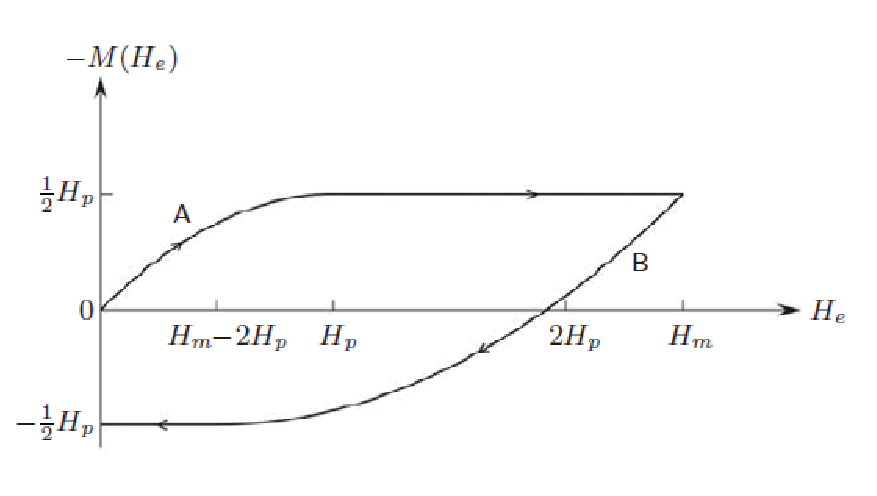
\includegraphics[scale=0.7]{chpt7/figs/fig7.12.eps}
	\caption{“大”磁场激励下的$-M(H_e)$。$H_m\le 2H_p=2J_c a$。}
\end{figure}

\subsubsection{问题7.3之解}
a) 如在“小”磁场序列下一样,$E_z(x)$由S1.3给出,其中$x_-=(H_m-H_e)/2J_c$。这样,
$e_{hy2'}$可由S1.4给出,除了场范围是从$H_m$到$H_m-2H_p$:
\begin{align*}% 7.16a
e_{hy2'}=&\frac{\mu_0 J_c}{a}\int_{H_m}^{H_m-2H_p}\left[\int_{0}^{x_-}(x-x_-)dx\right]dH_e=-\frac{\mu_0 J_c}{a}\int_{H_m}^{H_m-2H_p} x_-^2 dH_e\\
=&-\frac{\mu_0}{8H_p}\int_{H_m}^{H_m-2H_p}(H_m-H_e)^2 dH_e=-\frac{\mu_0}{8H_p}\int_{H_m}^{H_m-2H_p}(H_m^2-2H_mH_e+H_e^2) dH_e\\
e_{hy2^\prime}=&\frac{1}{3}\mu_oH_{p}^{2} \tag{7.16a}
\end{align*}

b) 在$x_-=a$时,S1.3给出$E_z(x)$,S1.4给出$e_{hy2''}$:
\begin{align*}% 7.16b
e_{hy2''}=\frac{\mu_0 J_c}{a}\int_{H_m-2H_p}^{0}\left[\int_{0}^{a}(x-a)dx\right]dH_e=\frac{\mu_0J_c}{2a}\int_{H_m-2H_p}^{0}a^2 dH_e\\
e_{hy2^{\prime\prime}}=\frac{1}{2}\mu_oH_pH_m\left(1-\frac{2H_p}{H_m}\right) \tag{7.16b}
\end{align*}

c) 将$e_{hy2'}$和$e_{hy2''}$相加:
\begin{align*}% 7.14b
e_{hy}&=e_{hy2'}+e_{hy2''}\\
&=\frac{1}{3}\mu_0 H_p^2 +\frac{1}{2}\mu_0H_p H_m\left(1-\frac{2H_p}{H_m}\right)\\
e_{hy}&=\frac{1}{2}\mu_oH_pH_m\left(1-\frac{4H_p}{3H_m}\right)  \quad   (H_m\geq 2H_p) \tag{7.14b}
\end{align*}

d) 简单的将7.13b($H_e=0\rightarrow H_m$下的$e_{hy}$)和7.14b相加:
\begin{align*}% 7.15c
e_{hy}=\frac{1}{2}\mu_0 H_p H_m\left(1-\frac{2H_p}{3H_m}\right)+\frac{1}{2}\mu_0 H_p H_m\left(1-\frac{4H_p}{3H_m}\right)\\
e_{hy}=\mu_oH_pH_m\left(1-\frac{H_p}{H_m}\right) \quad   (H_m\geq 2H_p) \tag{7.15c}
\end{align*}

e) 在$H_m=2H_p$时,7.15b和7.15c均可给出$e_{hy}$:
\begin{align*}% 7.15b
e_{hy}=&\frac{1}{2}\mu_oH_pH_m\left[1-\frac{2H_p}{3H_m}+\frac{1}{12}\left(\frac{H_m}{H_p}\right)^2\right]\\\tag{7.15b}
=&\mu_oH_{p}^{2}\left(1-\frac{1}{3}+\frac{4}{12}\right)=\mu_oH_{p}^{2}
\end{align*}
\begin{align*}% 7.15c
e_{hy}&=\mu_oH_pH_m\left(1-\frac{H_p}{H_m}\right) \\\tag{7.15c}
&=2\mu_oH_{p}^{2}\left(1-\frac{1}{2}\right)=\mu_oH_{p}^{2}
\end{align*}

\subsection{讨论7.1:磁滞能量密度——磁化的Bean板(情况4-6)}
一旦置于外场中,无染的Bean板即使在磁场降至0后,仍有磁化---图7.4a、7.4b和7.4c中的方点线。

对一个如情况4$H_e=0\rightarrow H_m$中的磁化Bean板,$-M(H_e)$为:
\textbf{“小”}($H_e=0\rightarrow H_m$)
\begin{equation}% 7.17a
-M(H_e)=H_e-\frac{H_{e}^{2}+2H_mH_e-H_{m}^{2}}{4H_p}
\end{equation}

\textbf{“中”}($H_e=0\rightarrow 2H_p-H_m$)
\begin{align*}% 7.17b
-M(H_e)=-\frac{1}{2}H_p+(H_m+H_e)-\frac{(H_m+H_e)^2}{4H_p} \tag{7.17b}
\end{align*}

\textbf{“中”}($H_e=2H_p-H_m\rightarrow H_m$)和\textbf{“大”}($H_e=0\rightarrow H_m$)
\begin{align*}% 5.6
-M(H_e)=\frac{1}{2}H_p \tag{5.6}
\end{align*}

类似的,对情况5$H_e=H_m\rightarrow 0$,$-M(H_e)$为下面的函数中的一个:

\textbf{“小”}($H_e=H_m\rightarrow 0$)
\begin{equation}% 7.18
-M(H_e)=H_e+\frac{H_{e}^{2}+2H_mH_e-H_{m}^{2}}{4H_p}
\end{equation}

\textbf{“中”}($H_e=H_m\rightarrow 0$)和\textbf{“大”}($H_e=H_m\rightarrow H_m-2H_p$)
\begin{align*}% 5.7a
-M(H_e)=\frac{1}{2}H_p-(H_m-H_e)+\frac{(H_m-H_e)^2}{4H_p} \tag{5.7a}
\end{align*}

\textbf{“大”}($H_e=H_m-2H_p\rightarrow 0$)
\begin{align*}% 5.7b
-M(H_e)=-\frac{1}{2}H_p
\end{align*}

图7.13给出了磁场在$-H_m$到$H_m$范围内的$-M(H_e)$。
点画线、虚线和实线分别对应情况6中的“小”、“中”和“大”磁场路径。
\begin{figure}[htbp]
	\centering
	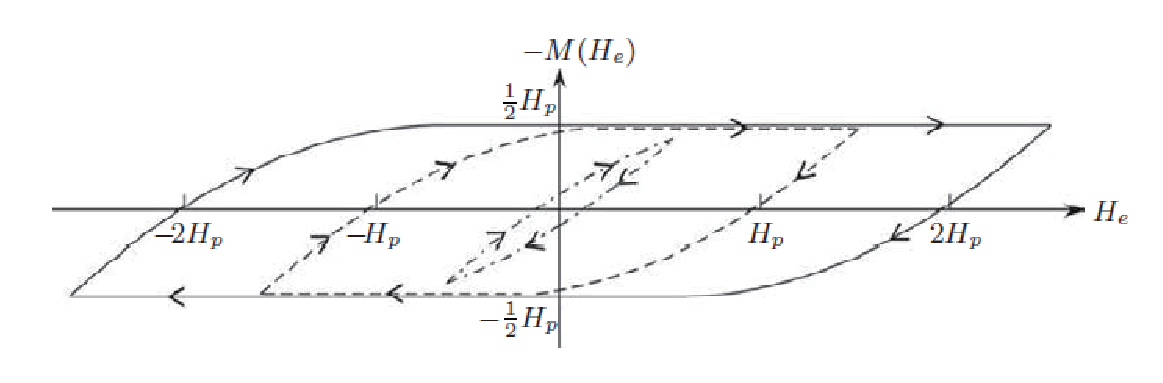
\includegraphics[scale=0.7]{chpt7/figs/fig7.13.eps}
	\caption{$-H_m$到$H_m$范围内的$-M(H_e)$图。}
\end{figure}

\textbf{情况4---“小”}\quad 可以使用问题7.1中的方法,其中$E_z(x)dt$有S1.1b给出:
\begin{align*}% page425 S1.1b
E_z(x)dt=\mu_oH(x_+-x)dH_e \tag{S1.1b}
\end{align*}
这里,如图7.4,$x_+=(H_m+H_e)/2J_c$而不是像问题7.1的$x_+=H_e/J_c$。
S1.1b可以导出S1.2c:
\begin{align*}% page425 S1.2c
e_{hy}=\frac{\mu_oJ_c}{a}\int_{0}^{H_m}\left(x_{+}^{2}-\frac{x_{+}^{2}}{2}\right)dH_e \tag{S1.2c}
\end{align*}
然后,将$x_+=(H_m+H_e)/2J_c$代入到S1.2c,有:
\begin{align*}% 7.19a两个
e_{hy}&=\frac{\mu_oJ_c}{2a}\int_{0}^{H_m}\left(\frac{H_m+H_e}{2J_c}\right)^2dH_e \\
&=\frac{\mu_o}{8H_p}\int_{0}^{H_m}(H_{m}^{2}+2H_mH_e+H_{e}^{2})dH_e\\
&e_{hy}=\frac{7\mu_oH_{m}^{3}}{24H_p} \quad(0\le H_m\le H_p) \tag{7.19a}
\end{align*}

\textbf{情况4---“中”}\quad 在图7.6b中可以看出,当$H_e$达到$H_e+H_m=2H_p$(即$H_e=2H_p-H_m$,记住此处$H_p\le H_m\le 2H_p$),通过板(从$x=0$到$x=a$)的$H_s=H_e-J_c x$。$E_z(x)$可由问题7.2解中的S2.2给出:
\begin{align*}% page425 S2.2
E_z(x)=\mu_o\frac{dH_e}{dt}(a-x) \tag{S2.2}
\end{align*}
直到$H_e=2H_p-H_m$,$H_e$仅穿透到$x_+$。这样,$e_{hy}$必须在$H_e=0\rightarrow 2H_p-H_m$和
$H_e=2H_p-H_m\rightarrow H_m$两个磁场范围内计算。分别使用S1.1b和S2.2的$E_z(x)dt$:
\begin{align*}% 7.19b
e_{hy}&=\frac{\mu_oJ_c}{2a}\left[\int_{0}^{2H_p-H_m}\left(\frac{H_m+H_e}{2J_c}\right)^2dH_e+\int_{2H_p-H_m}^{H_m}a^2dH_e\right] \\
&=\frac{\mu_o}{8H_p}\int_{0}^{2H_p-H_m}(H_{m}^{2}2H_mH_e+H_{e}^{2})dH_e+\frac{1}{2}\mu_oH_p\int_{2H_p-H_m}^{H_m}dH_e \\
&=\left(\frac{1}{3}\mu_oH_{p}^{2}-\frac{\mu_oH_{m}^{3}}{24H_p}\right)+(\mu_oH_pH_m-\mu_oH_{p}^{2}) 
\end{align*}
于是,
\begin{align*}
e_{hy}=\mu_oH_pH_m\left[1-\frac{2H_p}{3H_m}-\frac{1}{24}\left(\frac{H_m}{H_p}\right)^2\right]      (H_p\leq H_m\leq 2H_p)
\end{align*}
显然,7.19a和7.19b在$H_m=H_p$时自洽:$e_{hy}=7\mu_0 H_p^2/24$。

\textbf{情况4---“大”}\quad 如图7.4c可见,整个场范围内都会穿透整个板。于是:
\begin{align*}% 7.19c两个
e_{hy}=&\frac{\mu_oJ_c}{2a}\left(\int_{0}^{H_m}a^2dH_e\right)=\frac{1}{2}\mu_oH_p\int_{0}^{H_m}dH_e
e_{hy}=&\frac{1}{2}\mu_oH_pH_m \quad (H_m\geq 2H_p) \tag{7.19c}
\end{align*}
同样,7.19b和7.19c在$H_m=2H_p$时给出同样的结果:$e_{hy}=\mu_0 H_p^2$。

\textbf{情况5---“小”}\quad 对比情况2下的图7.4和7.3,我们发现情况5下的$H_s(x)$在“小”、“中”、“大”场
时和情况2对应的$H_s(x)$是一致的;
所以,情况5下的$e_{hy}$与情况2对应相同。

\textbf{情况6---“小”}\quad $e_{hy}$显然是对情况2“小”场成立的7.19a和7.14a之和的两倍:
\begin{align}% 7.20a两个
e_{hy}=&2\times7\left(\frac{7\mu_oH_{m}^{3}}{24H_p}+\frac{\mu_oH_{m}^{3}}{24H_p}\right)\\\notag
e_{hy}=&\frac{2\mu_oH_{m}^{3}}{3H_p}     (0\leq H_m\leq H_p)
\end{align}
当然,因为磁场会经过一个完整的周期,我们可以使用7.4b从7.20中得到$e_{hy}$。
因为$-M(H_e)$是反对称的,$-H_m$到$H_m$的积分等于从0到$H_m$的积分的两倍:
\begin{align*}% 7.4b和7.21
e_{hy}&=\mu_o\oint-M(H_e)dH_e \\
&=2\mu_o\int_{0}^{H_m}-M(H_e)dH_e\\ 
&=2\mu_o\int_{0}^{H_m}\{-[M(H_e)]_{H_e=0\rightarrow H_m}+[M(H_e)]_{H_e=H_m\rightarrow 0}\}dH_e \tag{7.21}
\end{align*}
将71.7a和7.18代入7.21,有:
\begin{align*}% 7.20a两个
e_{hy}=&2\mu_o\int_{0}^{H_m}\big[\left(H_e-\frac{H_{e}^{2}+2H_mH_e-H_{m}^{2}}{4H_p}\right) \\
&-\left(H_e+\frac{H_{e}^{2}-2H_mH_e-H_{m}^{2}}{4H_p}\right)\big]dH_e \\
=&2\mu_o\int_{0}^{H_m}\left(-\frac{H_{e}^{2}}{2H_p}+\frac{H_{m}^{2}}{2H_p}\right)dH_e=2\mu_o\left(-\frac{H_{m}^{3}}{6H_p}+\frac{H_{m}^{3}}{2H_p}\right)
\end{align*}
所以,
\begin{align*}
e_{hy}=\frac{2\mu_oH_{m}^{3}}{3H_p} \quad (0\leq H_m\leq H_p) \tag{7.20}
\end{align*}

\textbf{情况6---“中”}\quad 类似的,$e_{hy}$为对情况4成立的7.19b和对情况2(和5)成立的7.14a对应的$e_{hy}$之和的两倍:
\begin{align*}% page427 前7.20b两个
e_{hy}&=2\times\{\mu_oH_pH_m\left[1-\frac{2H_p}{3H_m}-\frac{1}{24}\left(\frac{H_m}{H_p}\right)^2\right]+\frac{\mu_oH_{m}^{3}}{24H_p}\}\\
e_{hy}&=2\mu_oH_pH_m\left(1-\frac{2H_p}{3H_m}\right)\quad (H_p\leq H_m\leq 2H_p) \tag{7.20b}
\end{align*}
我们可以由与7.4a等价的7.21推导出上式:
\begin{align*}% 7.21
e_{hy}=-2\mu_o\int_{0}^{H_m}\{[M(H_e)]_{H_e=0\rightarrow H_m}-[M(H_e)]_{H_e=H_m\rightarrow 0}\}dH_e \tag{7.21}
\end{align*}
因为$-M(H_e)$在$H_e=0\rightarrow 2H_p-H_m$时由71.7b给出,在$H_e=2H_p-H_m\rightarrow H_m$时
由5.6给出,7.21的积分包括两个部分。将7.17b、5.6和5.7a代入7.21,有:
\begin{align*}% page427倒数第二个
e_{hy}=&2\mu_o\{\int_{0}^{2H_p-H_m}\left[-\frac{1}{2}H_p+(H_m+H_e)-\frac{(H_m+H_e)^2}{4H_p}\right]dH_e \\
&+\int_{2H_p-H_m}^{H_m}\frac{1}{2}H_pdH_e-\int_{0}^{H_m}\left[\frac{1}{2}H_p-(H_m-H_e)+\frac{(H_m-H_e)^2}{4H_p}\right]\}dH_e\\
=&2\mu_o\{\int_{0}^{2H_p-H_m}\left[-\frac{1}{2}H_p+H_m+H_e-\frac{H_{m}^{2}}{4H_p}-\frac{H_mH_e}{2H_p}-\frac{H_{e}^{2}}{4H_p}\right]dH_e \\
&+H_p(H_m-H_p)-\int_{0}^{H_m}\left[\frac{1}{2}H_p-H_m+H_e+\frac{H_{m}^{2}}{4H_p}-\frac{H_mH_e}{2H_p}+\frac{H_{e}^{2}}{4H_p}\right]\}dH_e \\
=&2\mu_o\big[\left(\frac{1}{3}H_{p}^{3}+\frac{1}{2}H_pH_m-\frac{1}{2}H_{m}^{2}+\frac{H_{m}^{3}}{12H_p}\right)\big] \\
=&2\mu_o\left(-\frac{2}{3}H_{p}^{2}+H_pH_m\right) 
\end{align*}
于是,
\begin{align*}
e_{hy}=2\mu_oH_pH_m\left(1-\frac{2H_p}{3H_m}\right)\quad (H_p\leq H_m\leq 2H_p) \tag{7.20b}
\end{align*}

\textbf{情况6---“大”}\quad 这里同样,$e_{hy}$是为对情况4成立的7.19c和对情况2(和5)成立的7.14b对应的
$e_{hy}$之和的两倍:
\begin{align*}% page428 7.20c两个
e_{hy}=2\times\left[\frac{1}{2}\mu_oH_pH_m+\frac{1}{2}\mu_oH_pH_m\left(1-\frac{4H_p}{3H_m}\right)\right]\\
e_{hy}=2\mu_oH_pH_m\left(1-\frac{2H_p}{3H_m}\right) \quad (H_m\geq 2H_p) \tag{7.20c}
\end{align*}

方程7.20c也可以由7.21导出。同样,尽管5.6给出的是对增长序列(情况4)的全磁场范围的$-M(H_e)$,但因为在减小场序列(情况5)
中,5.7a给出的是$H_e=H_m\rightarrow H_m-2H_p$范围的,5.7b给出的是$H_e=H_m-2H_p\rightarrow 0$范围的,这导致
7.21的积分包括三个部分:
\begin{align*}% page428 7.21和7.20c合成的
e_{hy}=&2\mu_o\int_{0}^{H_m}\{-[M(H_e)]_{H_e=0\rightarrow H_m}+[M(H_e)]_{H_e=H_m\rightarrow 0}\}dH_e \\\tag{7.21}
=&2\mu_o]\big\{\int_{0}^{H_m}\frac{1}{2}H_pdH_e 
-\int_{H_m-2H_p}^{H_m}\left[\frac{1}{2}H_p-(H_m-H_e)+\frac{(H_m-H_e)^2}{4H_p}\right]\\
&-\int_{0}^{H_m-2H_p}(-\frac{1}{2}H_p)\big\}dH_e\\ 
=&2\mu_o\big[H_p(H_m-H_p)\\ 
&+\int_{H_m-2H_p}^{H_m}\left(-\frac{1}{2}H_p+H_m-\frac{H_{m}^{2}}{4H_p}-H_e+\frac{H_mH_e}{2H_p}-\frac{H_{e}^{2}}{4H_p}\right)dH_e\big] \\
=&2\mu_o[H_p(H_m-H_p)+\frac{1}{3}H_{p}^{2}]
\end{align*}
\begin{align*}
e_{hy}=2\mu_oH_pH_m\left(1-\frac{2H_p}{3H_m}\right)   \quad  (H_m\geq 2H_p) \tag{7.20c}
\end{align*}

注意到$H_m\gg H_p$(这是多数应用中一般能满足的条件)时,$e_{hy}$正比于$H_m$;
因为$H_p=J_c a$,$e_{hy}$也随$J_c$和$a$增长:
\begin{align*}% 7.20d和7.20e
e_{hy}=2\mu_oH_pH_m \quad  (H_m\gg H_p) \tag{7.20d}
\end{align*}
\begin{align*}
e_{hy}=2\mu_oJ_caH_m \quad (H_m\gg H_p) \tag{7.20e}
\end{align*}


\subsection{讨论7.2:载有直流电流的Bean板}
当传输电流$I_t$在$2a$宽度的Bean板中沿$z$方向均匀分布流动时,板内的$y$向磁场分布$H_s(x)$
不再关于板的中点镜像对称,如第五章的图5.5。
注意到$I_t$是$y$方向上单位长度的电流,单位为安培/米[A/m]。
将$i$定义为归一化传输电流:$i= I_t / I_c$,其中$I_c = 2a J_c$ [A / m]。 我们将研究暴露于外场$H_e(t)$的载流Bean板中的$H_s(x)$的分布。

\textbf{情况1i和2i}

我们从情况1i和2i时间序列开始---由公式7.5给出。
情况1i和2i中所选实例的$H_x(t)$曲线如7.14(a)-(d)所示。
在每个图中,点线和虚线分别对应于每个场序列的开始($H_e = 0$)和结束($H_e = H_m$)的$H_s(x)$。
注意到,图(a)和(b)中的点线在将在$I_t$施加“无染”板后给出$H_s(x)$;
浅虚线是在没有传输电流的情况时,在$H_e(t)=H_p$和$2H_p$的$H_s(x)$。
图(a)-(d)用于情况1i和2i; 图(a)和(b)是$H_m<H_p(1-i)$下的,而图(c)和(d)是$H_m> H_p(1-i)$下的。
当$H_m = H_p(1-i)\equiv H_m^*$时,(c)和(d)中的点划线对应于每个序列结束时的$H_s(x)$。
\begin{figure}[htbp]
	\centering
	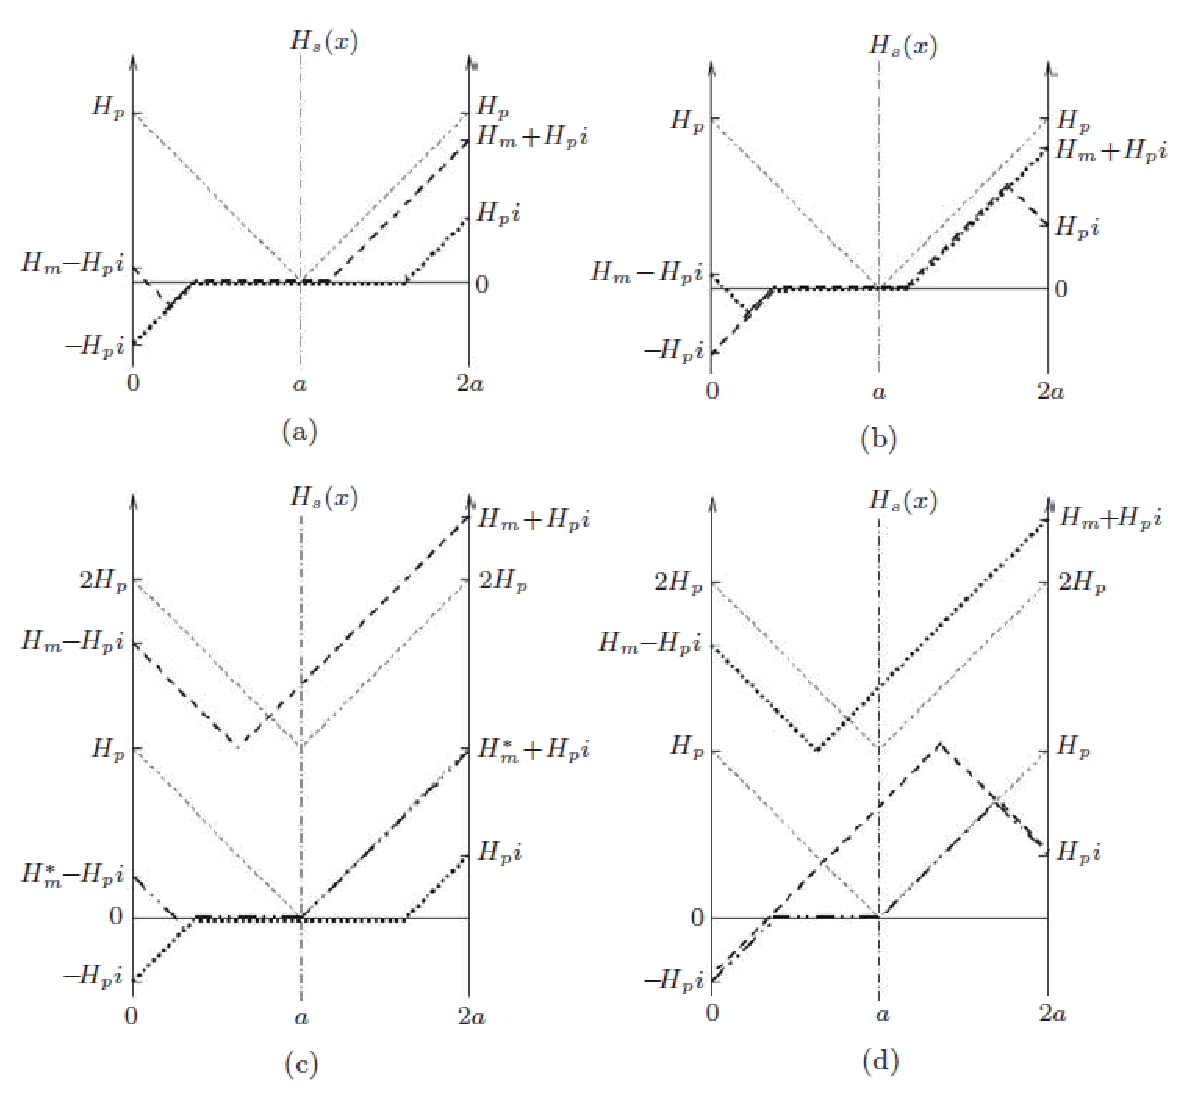
\includegraphics[scale=0.7]{chpt7/figs/fig7.14.eps}
	\caption{Graphs of Hs(x) plots for a Bean slab of width 2a carrying DC transport
		current of It(=2iHp), subjected to He(t) of Cases 1i and 2i, where Hm is the maximum
		external field. 。}
\end{figure}

\textbf{情况4i和5i---"小"磁场激励}

我们现在考察情况4i和5i的$H_s(x)$,如图7.15所示,其中外场$H_e(t)$的最大幅值$H_m$是“小”的,
具体而言,$H_m\le H_p(1-i)$。
从图中可以看出,因为场分布相对于板的中点是不对称的,所以稍后当计算磁滞能量密度时,
水平距离是可以从左端$x = 0$($x$轴)也可以从右端$xi= 0$($\xi$轴,即$x=2a$)测量---
两种方法下,场分布均由$H_x(x)$指定。
图(a)用于外场增加($\uparrow H_e$)序列的情况4i,即在场序列$H_e(t)=-H_m\rightarrow 0$之后
有$H_e(t)= 0\rightarrow H_m$;
图(b)用于外场减小($\downarrow H_e$)序列的情况5i,即$H_e(t)= H_m\rightarrow 0$。
在每个图中,点线和虚线分别对应于在场序列的开始和结束时的$H_s(x)$;
实线是$H_s(x)$在$0<\uparrow H_e<H_m$(情况4i)或$H_m>\downarrow H_e> 0$(情况5i)。

\begin{figure}[htbp]
	\centering
	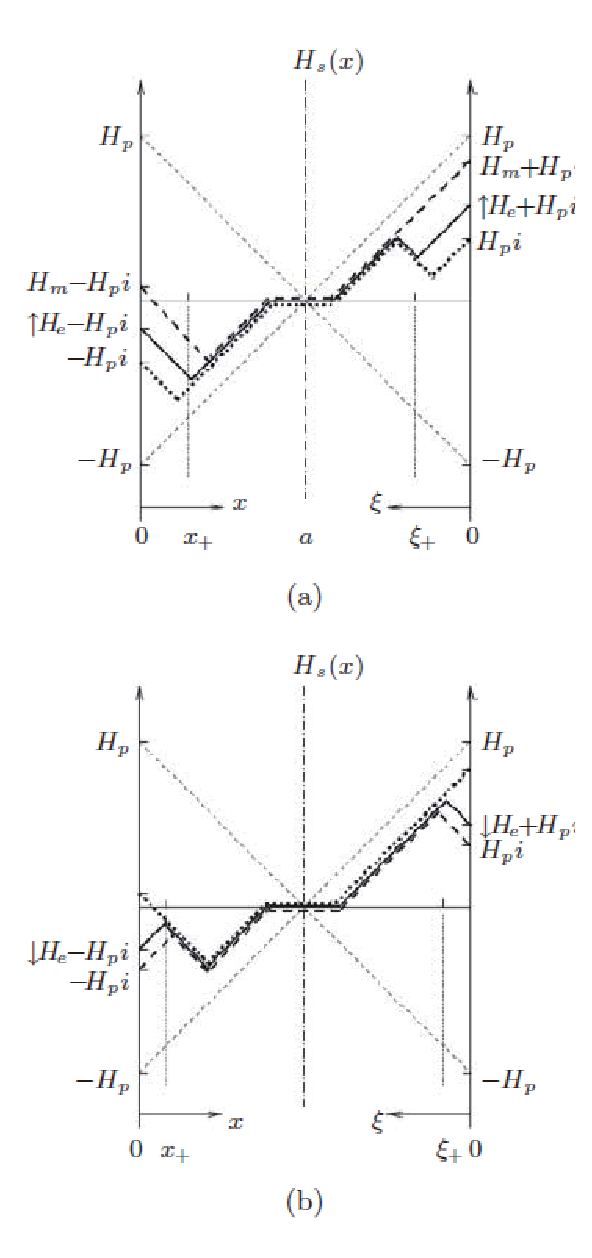
\includegraphics[scale=0.7]{chpt7/figs/fig7.15.eps}
	\caption{Hs(x) plots for Cases 4i and
		5i, in which Hm ≤ Hp(1−i). 。}
\end{figure}

\textbf{情况4i和5i---"大"磁场激励}

接下来,我们考察情况4i和5i在$H_m$是“大”的,即$H_m\ge 2H_p(1-i)$时的$H_s(x)$。
同样,$x$轴和$\xi$轴都会使用。
在每个图中,点线和虚线分别对应于场序列的开始和结束处时的$H_s(x)$。
图(a)是在场序列$H_e(t)= -H_m\rightarrow 0$之后的情况4i。
从一开始,场即从两侧完全穿透板,$H_m> H_p(1-i)$。
这里,$x$轴上有$\ell^*= a(1-i)$,$\xi$轴上的有$\ell^*= a(1+a)$;
实线用于$0 <\uparrow H_e <H_m$时的$H_s(x)$,该场分布在$0\le H_e\le H_m$时保持不变。

图(b)用于情况5i的减小场序列,其中$\downarrow H_e$直到它从$H_m$减小到$H_m^*$第没有完全穿透板。
$H_m^*$由$H_m^*= H_m -2H_p(1-i)$给出。
$\downarrow H_e = H_m^*$时的$H_s(x)$由点划线绘制;
$H_s(0)= H_m^* -H_p i$,$H_s(\xi_0)= H_m^* + H_p i$;
图中的点划线对应于$H_m^*\le He\le H_m$的$H_s(x)$。

对于$\downarrow H_e^*\equiv H_e\le H_m^*$,场完全穿透,
实线对应于场序列其余部分的$\downarrow H_e^*$。
这里,从图(b)可以推断,$x$轴上$\ell^* = a(1+i)$,$\xi$轴上$\ell^* = a(1-i)$。

注意到,情况5i中在完全穿透时$H_s(x)$是情况4i的镜像。
\begin{figure}[htbp]
	\centering
	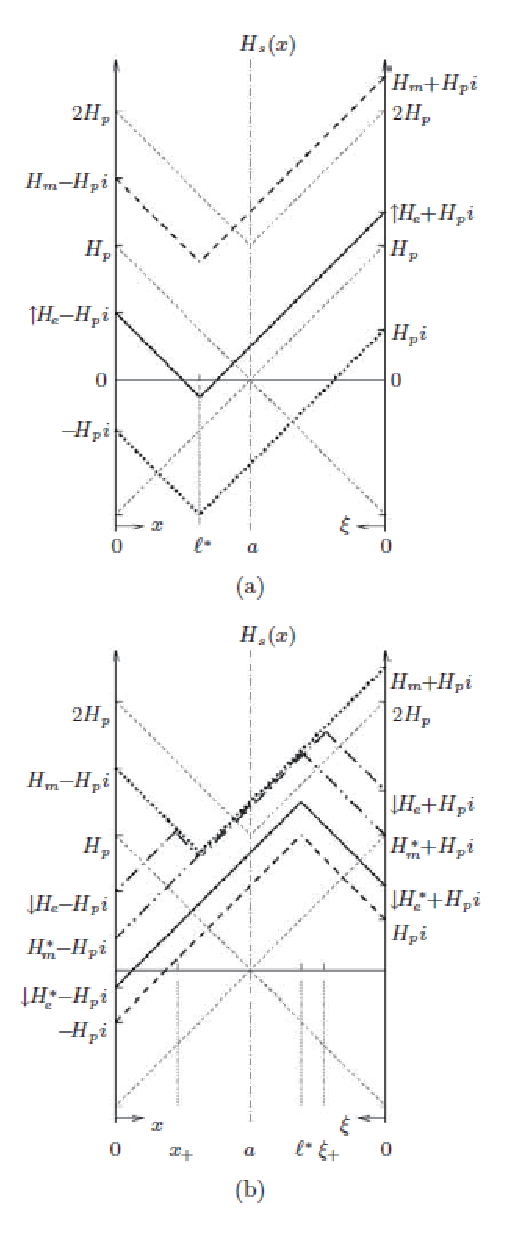
\includegraphics[scale=0.7]{chpt7/figs/fig7.16.eps}
	\caption{Hs(x) plots for Cases 4i and
		5i, in which Hm ≥ 2Hp(1−i). 。}
\end{figure}



\subsection{问题7.4:磁滞能量密度——载有直流电流的Bean板(情况4i--6i)}
在这里,我们研究承载DC传输电流$I_t$(沿$y$方向单位长度)在$y$向外施均匀磁场$H_e(t)$下的
Bean板在4i-6i的时间序列下的磁滞耗散。
如上所述,$I_t$也可以表示为$H_pi$,其中$i\equiv I_t/ I_c$。
使用7.3a中的$J_c E(x)dt$方法导出下面的$e_{hy}$表达式。

a) 证明情况4i$H_e=0\rightarrow H_m$在“小”磁场偏移($H_m\le H_p(1-i)$)
下的磁滞能量密度为:
\begin{equation}% 7.22a
e_{hy}=\frac{7\mu_oH_{m}^{3}}{24H_p} \quad  [0\leq H_m\leq H_p(1-i)]
\end{equation}

b) 证明情况5i$H_e=H_m\rightarrow 0$在“小”磁场($H_m\le H_p(1-i)$)偏移
施加之后的磁滞能量密度为:
\begin{align*}% 7.22b
e_{hy}=\frac{\mu_oH_{m}^{3}}{24H_p} \quad   [0\leq H_m\leq H_p(1-i)] \tag{7.22b}
\end{align*}

c) 证明情况6i$H_e=0\rightarrow H_m\rightarrow 0\rightarrow -H_m\rightarrow 0$
在“小”磁场偏移($H_m\le H_p(1-i)$)后的磁滞能量密度为:
\begin{align*}% 7.22c
e_{hy}=\frac{2\mu_oH_{m}^{3}}{3H_p} \quad  [0\leq H_m\leq H_p(1-i)] \tag{7.22c}
\end{align*}
注意到7.22c给出的$e_{hy}$和7.20a给出的无载流板情况下的是一致的:在“小”磁场偏移下,
传输电流对磁滞损耗没影响。

d) 证明情况4i$H_e=0\rightarrow H_m$在“大”磁场偏移($H_m\ge 2H_p(1-i)$)下
的磁滞能量密度为:
\begin{equation}% 7.23a
e_{hy}=\frac{1}{2}\mu_oH_pH_m(1+i^2) \quad [H_m\geq2H_p(1-i)]
\end{equation}

e) 证明情况5i$H_e=H_m\rightarrow 0$在“大”磁场偏移($H_m\ge 2H_p(1-i)$)后
的磁滞能量密度为:
\begin{align*}% 7.23b
e_{hy}=\frac{1}{2}\mu_oH_pH_m(1+i^2)-\frac{2}{3}\mu_oH_{p}^{2}(1-i^3) \quad [H_m\geq2H_p(1-i)]\tag{7.23b}
\end{align*}

f) 证明情况6i$H_e=0\rightarrow H_m\rightarrow 0\rightarrow -H_m\rightarrow 0$
在“大”磁场偏移($H_m\ge 2H_p(1-i)$)下后的磁滞能量密度为:
\begin{equation}% 7.23c
e_{hy}=2\mu_oH_pH_m(1+i^2)-\frac{4}{3}\mu_oH_{p}^{2}(1-i^3)\quad  [H_m\geq2H_p(1-i)] \tag{7.23c}
\end{equation}

g) 证明72.3c在没有传输电流($i=0$)时退化为板内无传输电流的7.20c。


\subsubsection{问题7.4之解}
a) 首先推导在$H_s(x)$下板的$x$侧的磁滞能量密度$e_{hyx}$;$H_s(0)=\uparrow H_e-H_p i$,如图7.15a所示。
在板内的$x=0$和$x=x_+$之间,代入$x_+=(H_m+H_e)/2J_c$,由$dH_e/dt$感应出的$E_z(x)$为:
\begin{align*}% page433 S4.1a
E_z(x)=\mu_o\frac{dH_e}{dt}(x_+-x) \tag{S4.1a}
\end{align*}
\begin{align*}% page433 S4.1b
E_z(x)dt=\mu_o(x_+-x)dH_e \tag{S4.1b}
\end{align*}
联立S4.1b和7.3a,我们得到$0\le x\le a$半板的表达式:
\begin{align*}% 7.3a和S4.2a
e_{hyx}&=\frac{1}{2a}\int_{0}^{a}\left[\int J_cE(x)dt\right]dx\\
&=\frac{\mu_oJ_c}{2a}\int_{0}^{H_m}\left[\int_{0}^{x_+}(x_+-x)dx\right]dH_e \tag{S4.2a}
\end{align*}
代入入$x_+=(H_m+H_e)/2J_c$并积分,有:
\begin{align*}% page433 S4.2b
e_{hyx}=\frac{7\mu_oH_{m}^{3}}{48H_p} \tag{S4.2b}
\end{align*}

接下来,我们推导在$H_s(\xi)$下板的$\xi$侧磁滞能量密度$e_{hy\xi}$;$H_s(0)=\uparrow H_e+H_p i$,如图7.15a所示。
代入$\xi_+=(H_m+H_e)/2J_c$,很明显有$e_{hy\xi}=e_{hyx}$,因此$e_{hy}=2e_{eyx}$。从而:
\begin{align*}% 7.22a
e_{hy}=\frac{7\mu_oH_{m}^{3}}{24H_p}  \quad  [0\leq H_m\leq H_p(1-i)] \tag{7.22a}
\end{align*}

b) 考虑板的$x$侧。类似于S4.2a,$e_{hyx}$为:
\begin{align*}
e_{hyx}=\frac{\mu_0 J_c}{2a}\int_{H_m}^{0}\left[\int_{0}^{x^+}(x-x_+)dx\right]dH_e \tag{S4.3a}
\end{align*}
其中,在这个减小磁场序列中,$x_+=(H_m-H_e)/2J_c$。从而:
\begin{align*}% page433 S4.3a
e_{hyx}=\frac{\mu_oJ_c}{2a}\int_{H_m}^{0}x_{+}^{2}dH_e=-\frac{\mu_o}{16H_p}(H_m-H_e)^2dH_e  \tag{S4.3b}
\end{align*}
\begin{align*}
e_{hyx}=\frac{\mu_oH_{m}^{3}}{48H_p} \tag{S4.3c}
\end{align*}
同样,板的$\xi$侧和$x$侧的磁滞能量密度相同。因此,这个情况下的$e_{hy}$是S4.3c给出的$e_{hyx}$的两倍:
\begin{align*}% 7.22b
e_{hy}=\frac{\mu_oH_{m}^{3}}{24H_p}   \quad     [0\leq H_m\leq H_p(1-i)] \tag{7.22b}
\end{align*}

c) 情况6i的磁场序列包括$H_e(t)=0\rightarrow -H_m$和$H_e(t)=-H_m\rightarrow 0$,
其$e_{hy}$是情况4i和情况5i之和的二倍:
\begin{align*}% page434 S4.4
3_{hy}=2\times\left(\frac{7\mu_oH_{m}^{3}}{24H_p}+\frac{\mu_oH_{m}^{3}}{24H_p}\right) \tag{S4.4}
\end{align*}
由S4.4,我们有:
\begin{align*}% 7.22c
e_{hy}=\frac{2\mu_oH_{m}^{3}}{3H_p} \quad [0\leq H_m\leq H_p(1-i)] \tag{7.22c}
\end{align*}
如前所示,在“小”的磁场偏移($H_m\le H_p(1-i)$)下,
$e_{hy}$与板内的传输电流无关。

d) 首先考虑板内的$x$侧。和S4.2a类似,有:
\begin{align*}% page434 S4.5a
e_{hyx}=\frac{\mu_oJ_c}{2a}\int_{0}^{H_m}\left[\int_{0}^{\ell^*}(\ell^*-x)dx\right]dH_e \tag{4.5a}
\end{align*}
其中,从$x=0$测量,$\ell^*=a(1-i)$。于是:
\begin{align*}% page434 S4.5b
e_{hyx}=\frac{\mu_oJ_ca^2(1-i)^2}{4a}\int_{0}^{H_m}dH_e=\frac{1}{4}\mu_oH_pH_m(1-i)^2 \tag{S4.5b}
\end{align*}
接下来,考虑$\xi$侧。类似S4.2a,有:
\begin{align*}% page434 S4.6a
e_{hy\xi}=\frac{\mu_oJ_c}{2a}\int_{0}^{H_m}\left[\int_{0}^{\ell^*}(\ell^*-\xi)d\xi\right]dH_e \tag{S4.6a}
\end{align*}
其中,从$\xi$测量,$\ell^*=a(1+i)$。于是:
\begin{align*}% page434 S4.6b
e_{hy\xi}=\frac{\mu_oJ_ca^2(1+i)^2}{4a}\int_{0}^{H_m}dH_e=\frac{1}{4}\mu_oH_pH_m(1+i)^2\tag{S4.6b}
\end{align*}
因为$e_{hy}=e_{hyx}+e_{hy\xi}$,联立S4.5b和S4.6b,有:
\begin{align*}% 7.23a
e_{hy}=\frac{1}{2}\mu_oH_pH_m(1+i^2) \quad [H_m\geq 2H_p(1-i)] \tag{7.23a}
\end{align*}

e) 对情况5i这样的减小磁场序列,我们首先考虑$H_m$到$H_m^*\equiv H_m-2H_p(1-i)$区间。
考虑板的$x$侧,有:
\begin{align*}% page434 S4.7a
e_{hyx}=\frac{\mu_oJ_c}{2a}\int_{H_m}^{H_{m}^{*}}\left[\int_{0}^{x_+}(x-x_+)dx\right]dH_e \tag{S4.7a}
\end{align*}
式中,$x_+=(H_m-H_e)/2J_c$。于是:
\begin{align*}% page434 S4.7b
e_{hyx}&=\frac{\mu_oJ_c}{2a}\int_{H_{m}^{*}}^{H_m}\left(\frac{H_m-H_e}{2J_c}\right)^2dH_e \\\tag{S4.7b}
&=\frac{\mu_o}{16H_p}(H_{m}^{2}H_e-H_mH_{e}^{2}+\frac{1}{3}H_{e}^{3})\mid_{H_m-2H_p(1-i)}^{H_m} \\
&=\frac{1}{6}\mu_oH_{p}^{2}(1-i)^3
\end{align*}
从图7.16a可以清晰看出$e_{eyx}=e_{hy\xi}$,于是在
$H_e=H_m\rightarrow H_m-2H_p(1-i)$序列下,$e_{hy}$为:
\begin{align*}% page435 S4.7c
e_{hy}=\frac{1}{3}\mu_oH_{p}^{2}(1-i)^3 \tag{S4.7c}
\end{align*}
接下来,考虑序列$H_e=H_m^*\rightarrow0$。在$x$侧,有:
\begin{align*}% page435 S4.8a
e_{hyx}&=\frac{\mu_oJ_c}{2a}\int_{H_{m}^{*}}^{0}\left[\int_{0}^{x_+}(x-x_+)dx\right]dH_e=-\frac{\mu_oH_p(1+i)^2}{4}\int_{H_{m}^{*}}^{0}dH_e \\
&=\frac{1}{4}\mu_oH_p(1+i)^2[H_m-2H_p(1-i)] \\
&=\frac{1}{4}\mu_oH_pH_m(1+i)^2-\frac{1}{2}H_{p}^{2}(1+i)^2(1-i) \tag{S4.8a}
\end{align*}
在$\xi$侧,我们发现$e_{hy\xi}$非常类似于S4.8a:
\begin{align*}% page435 S4.8b
e_{hy\xi}=\frac{1}{4}\mu_oH_pH_m(1-i)^2-\frac{1}{2}H_{p}^{2}(1-i)^3 \tag{S4.8b}
\end{align*}
在$H_m-2H_p(1-i)$到0的区间,我们有$e_{hy}=e_{hyx}+e_{hy\xi}$;
联立S4.8a和S4.8b,有:
\begin{align*}% pge435 S4.8c
e_{hy}=\frac{1}{2}\mu_oH_pH_m(1+i^2)-\mu_oH_{p}^{2}(1-i)(1+i^2) \tag{S4.8c}
\end{align*}
情况5i的$e_{hy}$是方程S4.7c和S4.8c给出的之和:
\begin{align*}% 7.23b
e_{hy}=\frac{1}{2}\mu_oH_pH_m(1+i^2)-\frac{2}{3}\mu_oH_{p}^{2}(1-i^3) \quad [H_m\geq H_p(1-i)] \tag{7.23b}
\end{align*}

f) 情况6i($H_m\ge H_p(1-i)$)的$e_{hy}$是情况4i和情况5i给出的$e_{hy}$之和的两倍,包括$H_e(t)=0\rightarrow-H_m$
和$H_e(t)=-H_m\rightarrow 0$两个序列:
\begin{align*}% page435 S4.9
e_{hy}=2\times\left[\frac{1}{2}\mu_oH_pH_m(1+i^2)+\frac{1}{2}\mu_oH_pH_m(1+i^2)-\frac{2}{3}\mu_oH_{p}^{2}(1-i^3)\right] \tag{S4.9}
\end{align*}
由S4.9,可得:
\begin{align*}% 7.23c
e_{hy}=2\mu_oH_pH_m(1+i^2)-\frac{4}{3}\mu_oH_{p}^{2}(1-i^3) \quad [H_m\geq H_p(1-i)] \tag{7.23c}
\end{align*}

g) 将$i=0$代入7.23c,有:
\begin{align*}% page435 S4.10
e_{hy}=2\mu_oH_pH_m-\frac{4}{3}\mu_oH_{p}^{2} \tag{S4.10}
\end{align*}
我们注意到,S4.10和7.20b是等价的:
\begin{align*}% page435 7.20b
e_{hy}=2\mu_oH_pH_m\left(1-\frac{2H_p}{3H_m}\right) \tag{7.20b}
\end{align*}


\subsection{问题7.5:自场磁滞能量密度——Bean板}
当Bean板通过周期AC传输电流$I(t)$时,由于传输电流在板上产生周期AC表面场(外部)$H_e(t)$,它耗散能量。
单位体积的这种耗散称为自场磁滞能量密度$e_{sf}$。 电流--时间序列如下:
\begin{equation}% 7.25
I(t)=0^*(\ \mathrm{Virgin slab})\rightarrow I_m\rightarrow 0\rightarrow -I_m\rightarrow 0\rightarrow I_m\rightarrow 0\rightarrow -I_m\rightarrow 0
\end{equation}
7.25中,$I_m$是周期AC电力路的幅值。情况1st-3sf均针对非$无染$Bean板。
情况3sf是$0\rightarrow I_m\rightarrow 0\rightarrow -I_m\rightarrow 0$。
图7.17给出了宽$2a$的Bean板的$H_s(x)$图,图(a)和(b)分别对应情况1sf和2sf,电流序列非别为:
情况1sf$i(t)=0\rightarrow i_m$,情况2sf$i\equiv I/I_c\le i_m\equiv I_m/I_c\le 1$。
如图缩回,$H_s(x)$是关于板中点反对称的:为了推导下面的$e_{hy}$表达式,仅考虑板的从$x=0$到$x=a$的一半。

a) 应用7.3a,证明情况1sf的$e_{sf}$为:
\begin{equation}% 7.26a
e_{sf}=\frac{7}{24}\mu_oH_{p}^{2}i_{m}^{3}
\end{equation}

b) 应用7.3a,证明情况2sf的$e_{sf}$为:
\begin{align*}% 7.26b
e_{sf}=\frac{1}{24}\mu_oH_{p}^{2}i_{m}^{3} \tag{7.26b}
\end{align*}

c) 应用7.3a,证明情况3sf的$e_{sf}$为:
\begin{align*}% 7.26c
e_{sf}=\frac{2}{3}\mu_oH_{p}^{2}i_{m}^{3} \tag{7.26c}
\end{align*}

d) 从7.20a推导出7.26c,$e_{hy}$对情况6("小"场)成立。
\begin{figure}[htbp]
	\centering
	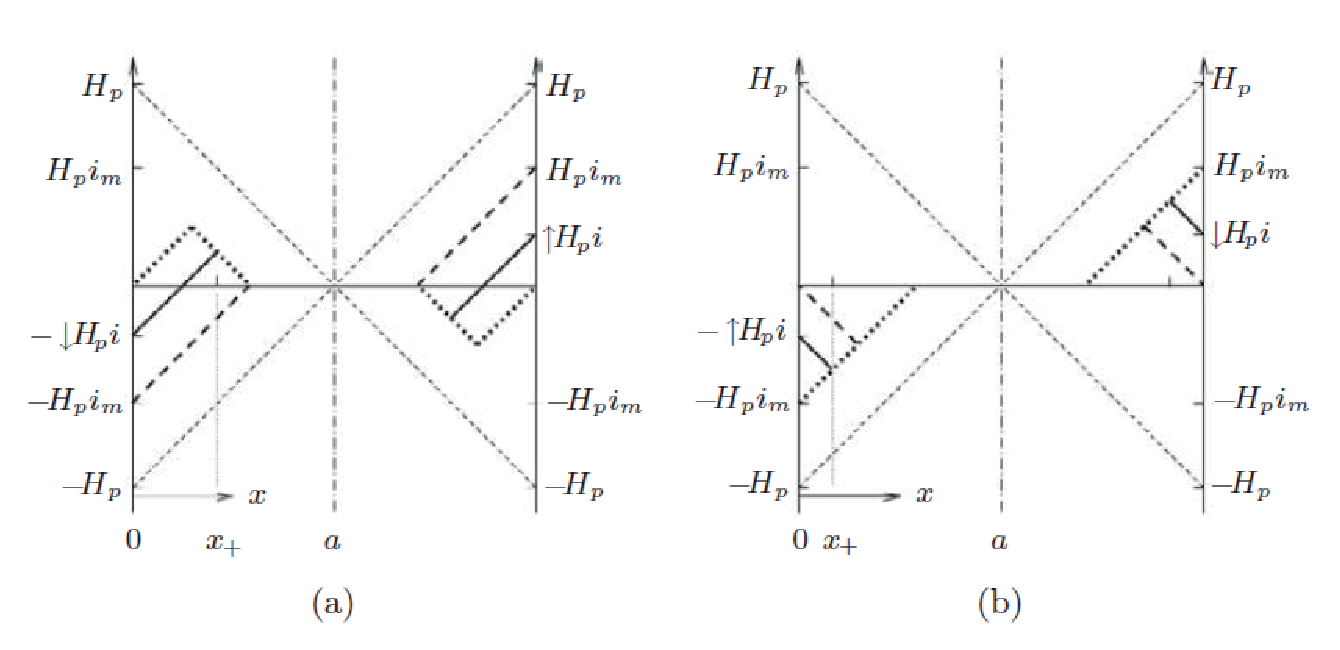
\includegraphics[scale=0.7]{chpt7/figs/fig7.17.eps}
	\caption{情况1sf和2sf下的$H_s(x)$图。(a)对应1sf;(b)对应2sf。各图中,点线和虚线分别对应电流序列
		开始和结束时的$H_s(x)$。}
\end{figure}


\subsubsection{问题7.5之解}
a) 对情况1sf,应用7.3a到$0\le x\le a$半板,随着传输电流从0增长到$i_m$,$x=0$自场$H_{sf}$从0减小到$-H_p i_m$:
\begin{align*}% page437 S5.1a和S5.1b
e_{sfx}=\frac{\mu_oJ_c}{2a}\int_{0}^{-H_pi_m}\left[\int_{0}^{x_+}(x-x_+)dx\right]dH_{sf}  \tag{S5.1a}
\end{align*}
\begin{align*}
e_{sfx}=\frac{\mu_oJ_c}{4a}\int_{0}^{-H_pi_m}(-x_{+}^{2})dH_{sf} \tag{S5.1b}
\end{align*}
将$H_{sf}=-H_p i$代入S5.1b,考虑$x_+=H_p(i_m+i)/2J_c$,我们得到:
\begin{align*}% page437 S5.2a和5.2b
e_{sfx}&=\frac{\mu_oH_{p}^{2}}{16}\int_{0}^{i_m}(i_{m}^{2}+2i_mi+i^2)di \\
&=\frac{7}{48}\mu_oH_{p}^{2}i_{m}^{3} \tag{S5.2}
\end{align*}
因为板的另一半($a\le x\le 2a$)有同等的耗散能量密度,情况1sf的$e_{sf}$是$e_{sfx}$的两倍:
\begin{align*}% 7.26a
e_{sf}=\frac{7}{24}\mu_oH_{p}^{2}i_{m}^{3} \tag{7.26a}
\end{align*}

b) 类似于情况1sf,情况2sf有$H_+=H_p(i_m-i)/2J_c$,于是:
\begin{align*}% page437 S5.3a和S5.3b和S5.3c
e_{sfx}&=\frac{\mu_oJ_c}{2a}\int_{-H_pi_m}^{0}\left[\int_{0}^{x_+}(x_+-x)dx\right]dH_{sf} \\
&=\frac{\mu_oH_{p}^{2}}{16}\int_{i_m}^{0}(i_{m}^{2}-2i_mi+i^2)di \\
&=\frac{1}{48}\mu_oH_{p}^{2}i_{m}^{3} \tag{S5.3c}
\end{align*}
这样,情况2sf的$e_{sf}$是S5.3给出的$e_{sfx}$的两倍:
\begin{align*}% 7.26b
e_{sf}=\frac{1}{24}\mu_oH_{p}^{2}i_{m}^{3} \tag{7.26b}
\end{align*}

c) 对情况3sf,因为其涵盖了完整周期,$e_{hy}$是情况1sf和情况2sf之和的两倍,
\begin{align*}% page437 S5.4
e_{sf}=2\times\left(\frac{7}{24}\mu_oH_{p}^{2}i_{m}^{3}+\frac{1}{24}\mu_oH_{p}^{2}i_{m}^{3}\right) \tag{S5.4}
\end{align*}
方程S5.4化简为:
\begin{align*}% 7.26c
e_{sf}=\frac{2}{3}\mu_oH_{p}^{2}i_{m}^{3} \tag{7.26c}
\end{align*}

d) 图7.17中的$H_p i_m$替换为$H_m$后,对磁滞能量密度计算而言,图7.17所示的场特征和对应情况4(“小”场)图7.4a所示的场特征是一致的。于是:
\begin{align*}% page438 7.20a和7.26c
e_{hy}&=\frac{2\mu_oH_{m}^{3}}{3H_p} \\ \tag{7.20a}
&=\frac{2\mu_o(H_pi_m)^3}{3H_p} 
\end{align*}
\begin{align*}
e_{hy}=\frac{2}{3}\mu_oH_{p}^{2}i_{m}^{3} \tag{7.26c}
\end{align*}


\subsection{讨论7.3:磁体整体的交流损耗}
表7.3-7.9总结的交流损耗能量密度闭式解仅适用于最简单的超导体配置和工况。
首先,超导体要是一个孤立的Bean板,其$J_c$是与场无关。
其次,施加的外磁场均匀且指向特定方向:平行于厚度($2a$)的Bean板的表面。
第三,如果存在传输电流,也是最简单的条件:当施加磁场时已经存在DC电流。

使用闭式分析表达式无法准确计算整个磁体的交流损耗。
如果必须知道磁体的总交流损耗,例如,估计系统制冷负荷,则最好采用数值计算技术将空间相关的“局部”交流损耗做累加。
对交流损耗的粗略估计,例如混合III超导磁体(问题7.7),则可以用表7.3-7.9中的表达式,
尽管导体配置和场/电流条件远比用于推导这些表达式的条件复杂得多。
由于存在时变场和传输电流,表达式并不普适。
对于短样和整个线圈,最可靠的方法是实测和数值分析的结合[7.1,7.2,7.4,7.61-7.85]。

不过应该注意的是,现在运行的绝大多数超导磁体都是绝热的(可能在不久的将来也是)。
绝热LTS或HTS磁体只能承受有限的交流损耗,限度为通过热传导可以将绕组最大温升$[\Delta T_{op}(I_{op})]_{st}$(温度裕度)
内的热量完全导出到外表面。这个温度裕度,HTS磁体通常大于LTS磁体。
为了估计这个峰值温度,计算绕组中可能具有最大值的小块区域一般就够了。
对于这种类型的计算,无需高精度,可以应用表7.3-7.9中的表达式。


\subsection{讨论7.4:测量交流损耗的技术}
如上所述,对于真实超导体,短样及整个磁体的交流损耗的精确计算几乎是不可能的:
唯一的依据是测量[7.61-7.103]。
有三种测量交流损耗的基本方法:1) 磁测法;;2) 量热法;3) 电测法。
磁测法仅适用于不带传输电流的“短”样(公式7.4b)的磁滞损耗(问题7.6)。
量热法将测试样品(短导体或甚至整个线圈)浸到制冷剂中(LTS为液氦,HTS为液氮),外施周期场和/或传输电流,
通过制冷剂的蒸发速率推导交流损耗;在该方法变体中,交流损耗引起的轻微温升用以确定损耗。
电测法是当测试样品通过时变传输电流$I_t(t)$时,测量时间积分$\int V(t)I_t(t)dt$,其中$V(t)$是测试样品上的电压。
实践中,测量$V(t)$时必须非常谨慎地设置电压抽头[7.98]。

\begin{figure}[htbp]
	\centering
	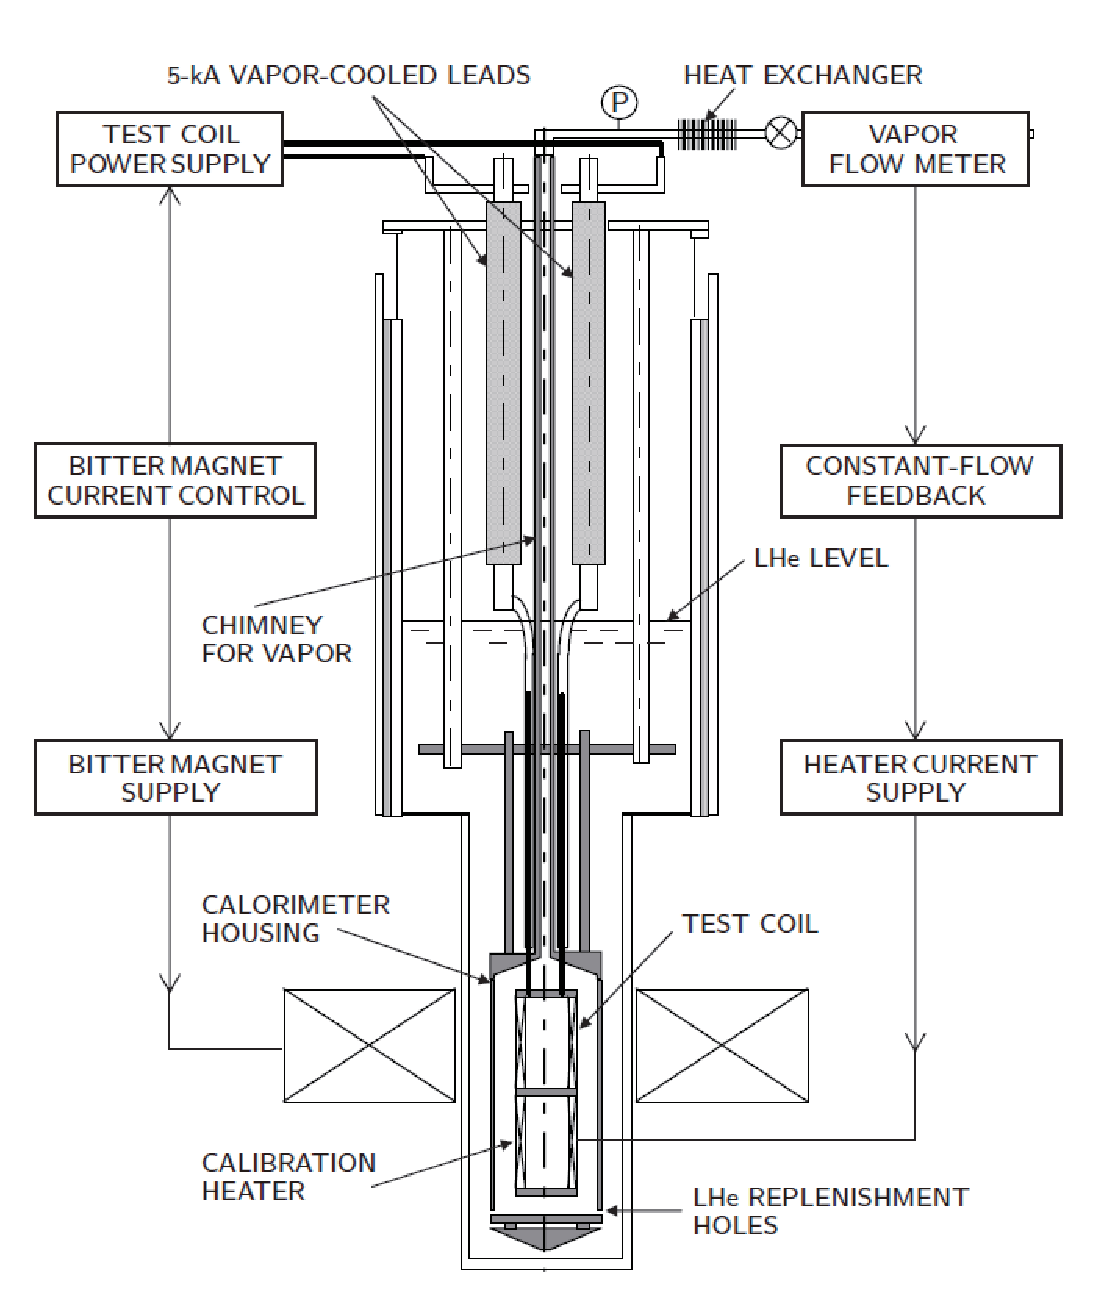
\includegraphics[scale=0.7]{chpt7/figs/fig7.19.eps}
	\caption{量热法测量置于时变磁场中、通过交流或直流超导测试线圈的交流损耗的试验装置的剖面示意图,基于原始图[7.
		87]。}
\end{figure}

图7.19给出了基于原始图[7.87]的用于测量超导测试线圈的总交流耗散的量热装置的截面示意图。
在量热法中,校准加热器放置在带有测试线圈的量热计外壳内,测试线圈通过交流或直流传输电流,时变外磁场由Bitter磁体
提供,控制校准加热器保持蒸发蒸汽率恒定,并用蒸汽流量计测量。
校准加热器输入的变化与测试线圈的总交流耗散有关。
为了稳定低温恒温器压力,在测量过程中不会补充液氦。
测试线圈和校准加热器流出的氦蒸汽通过通道导出,在室温环境下被整体流量计测量。
量热仪外壳底部有一组孔用以补充液氦,使容器充满液氦并维持低温恒温器压力。

\textbf{实例}\quad 这个测试线圈的总交流损耗是100-500 mW[7.87,7.88]。
液氦在4.22 K时的汽化潜热是$h_L=20.9$ kJ/kg(J/g);
4.22 K的100 mW耗散能量对应液氦汽化质量流量为4.8 mg/s或液体体积蒸发率0.038 $\mathrm{cm^3/s}$(密度1.25 $g/cm^3$)。
因为在大气压力下氦会膨胀,从4.22 K的液体到273 K的气体,膨胀倍数为700(附录II),
体积流量计测到的体积流量应为28.6 $cm^3/s$或1596 SCCM(standard(1 atm, 0$^\circ$C) cubic centimeter per minute, 标准立方米/分钟)

\subsection{讨论7.5:CICC中的交流损耗}
不同于超导体细丝嵌入导电基底中的导体,CIC导体因其股线可以是电磁解耦的而适用于交流应用。
(在这方面,Rutherford电缆也是如此,因为它的股线安装在高强度钢带上,同样可以去耦。)

与所有交流适用的股线一样,CIC导体的每股中的超导细丝被换位,并且每个细丝又被薄的“电阻”金属(常为Nb或Cu-Ni)隔离层包绕,
最小化的由时变条件感应的出的耦合电流。
隔离电阻越大,“有效Bean板厚度”和细丝间耦合时间常数$\tau_{cp}$(公式7.6)越小,
这分别意味着更小的磁滞能量密度$e_{hy}$和更小的耦合能量密度$e_{cp}$。

有效基底电阻率$\rho_{ef}$(公式7.7)决定了股线间耦合时间常数。
类似地,股线电阻率决定了股线间耦合时间常数,反过来股线间耦合时间常数又决定了股线间耦合能量密度。
对于CIC导体,股线间电阻率(或电阻)和耦合时间常数都需要测量[7.104-7.107]。

\subsection{讨论7.6:HTS中的交流损耗}
值得强调的是,HTS中交流损耗的机制与LTS中交流损耗的机制相同。
因此,为了使交流损耗最小化,必须:最小化HTS的尺寸(磁滞损耗);
超导细丝电磁去耦(耦合损耗);导电基底在超导体中少量添加(涡流损耗)。同时还应满足其他要求。

带材减小磁滞损耗效果最差的导体配置:于是,Bi2223,YBCO和MgB2(也可为导线)在某些交流应用中不适合。
尽管Bi2223和MgB2带包含许多“迷你”带以减小它们的有效尺寸(Bean板的$2a$),
但由于这些迷你带没有扭绞和换位,交流损耗仍然是一个关键问题;
对于YBCO已经提出减小有效尺寸并使微带分离的导体设计,虽然巧妙但可能难以经济地实现[7.108-7.113]。
对于一些交流应用,HTS线,如Bi2212和MgB2,可能更好。


\subsection{问题7.6:$Nb_3Sn$中的磁滞损耗}
本问题中我么考虑一种为聚变项目制造的$\mathrm{Nb_3 Sn}$导体。
图7.20给出了净直径为1.0,0.8,0.6,0.4,0.3 mm$\mathrm{Nb_3 Sn}/Cu$复合导体在4.2 K下测到的
$\mu_0 M$ vs. $\mu_0 H$图[7.114]。
\begin{figure}[htbp]
	\centering
	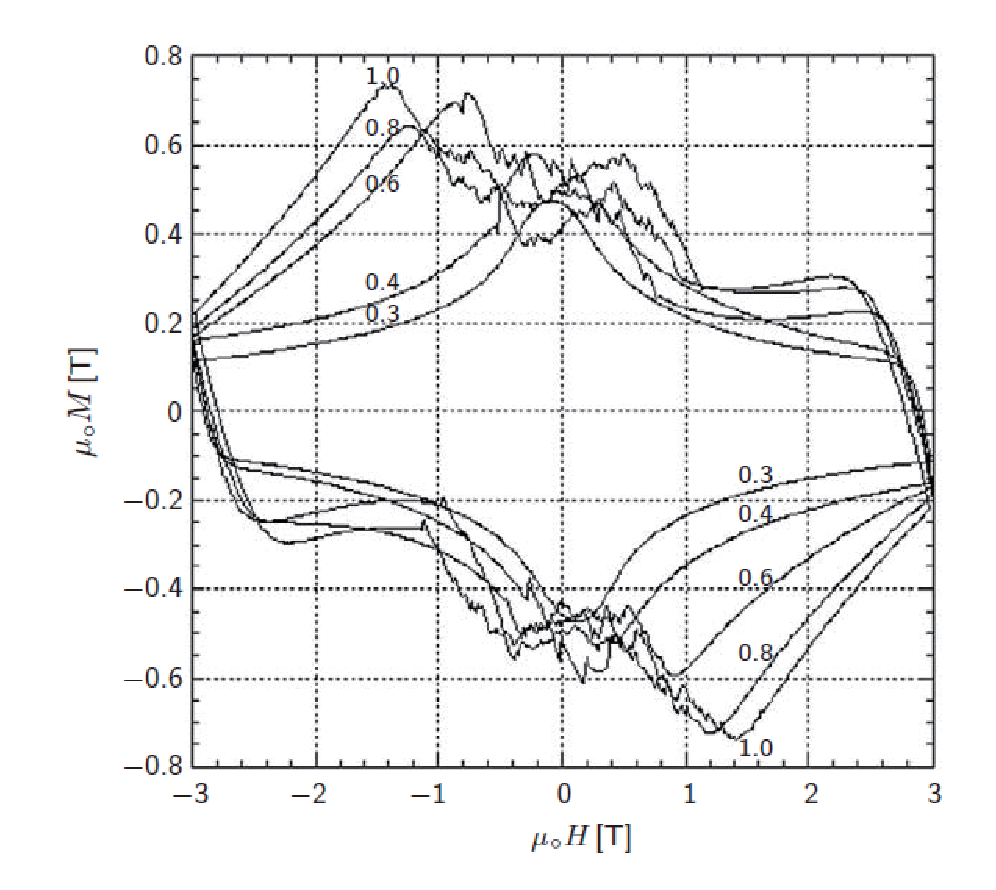
\includegraphics[scale=0.7]{chpt7/figs/fig7.20.eps}
	\caption{净直径为1.0,0.8,0.6,0.4,0.3 mm$\mathrm{Nb_3 Sn}/Cu$复合导体在4.2 K下测到的
		$\mu_0 M$ vs. $\mu_0 H$图。}
\end{figure}

a) $\phi$0.3 mm线(图7.20中的0.3)在3 T和4.2 K下的临界电流密度为$J_c$(3 T,4.2 K)=$0.72\times 10^{10}\ \mathrm{ A/m^2}$。证明,在$\pm 10\%$不确定度下,0 T时的临界电流$J_c$(0 T,4.2 K)=$2.8\times 10^{10}\ \mathrm{ A/m^2}$。
对$\mathrm{Nb_3 Sn}$导体,常假设$J_c=J_{noncu}$,即非同截面上的临界电流密度。

b) 假定线中的细丝都是圆截面的,计算0.3 mm线的有效细丝直径$d_{eff}$。
可以令$d_{eff}$等于Bean板的宽度$2a$。

c) 直径为0.8,0.6,0.4,0.3 mm的导线可以由1.0 mm的导线拉拔而成,故其细丝数目一样。
定型的解释图7.20中这些线的磁化曲线的两个重要差异。

d) 在一个$-3$ T到3 T的完整磁场周期内,计算$\phi$0.3 mm线的磁滞能量密度$e_{hy}$。
假定$B_p\ll$3 T。

\subsubsection{问题7.6之解}
a) 如图5.3所示的无磁通跳跃$M(\mu_0 H,T)$曲线所围区域正比于$J_c(\mu_0 H,T)$。
由7.20中$\phi$0.3 mm线的曲线可知,$|\mu_0$M(0 T,4.2 K)$|\simeq$0.47 T,
$|\mu_0$M(3 T,4.2 K)$|\simeq$0.12 T。于是:
\begin{align*}% page448第一个
J_c(0\ \mathrm{T},4.2\ \mathrm{K})&=J_c(3\ \mathrm{T},4.2\ \mathrm{K})\times\left| \frac{M(0\ \mathrm{T},4.2\ \mathrm{K})}{M(3\ \mathrm{T},4.2\ \mathrm{K})}\right| \\ 
&\simeq J_c(3\ \mathrm{T},4.2\ \mathrm{K})\times\frac{(0.47\ \mathrm{T})}{(0.12\ \mathrm{T})}\\
&\simeq J_c(3\ \mathrm{T},4.2\ \mathrm{K})\times 3.92 \\
&\simeq 2.8\times 10^{10}\ \mathrm{A/m^2}
\end{align*}

b) 根据Bean模型,在$H\ge H_p=J_c a$时,$M(H)=H_p/2$,使用$a=d_{eff}/2$,有:
\begin{align*}% page448第二个
M(H)=\frac{1}{2}H_p=\frac{1}{2}(d_{eff}/2)J_c(H)
\end{align*}
根据图7.20和问题a),我们分别有$\mu_0 M$(0 T)$\simeq$0.47 T和$J_c$(0 T)$\simeq 2.8\times 10^{10}\ \mathrm{ A/m^2}$。从而:
\begin{align*}% page448第三个
d_{eff}=\frac{4\mu_oM(0\ \mathrm{T})}{\mu_oJ_c(0\ \mathrm{T})}&\simeq\frac{4(470\times 10^{-3}\ \mathrm{T})}{(4\pi\times 10^{-7}\ \mathrm{H/m})(2.8\times10^{10}\ \mathrm{A/m^2})}\\
&=53\ \mathrm{\mu m}
\end{align*}
可见,当$M(H)$和$J_c(H)$均已知时,任意$H$值下的$d_{eff}$都是可以计算的。

c) 可从$-\mu_0 H=-$2 T时的正磁化幅值知道,幅值几乎在整个导线尺度上有$\propto d_{eff} J_c$。
这表明$d_{eff}$随导线直径减小而减小,尽管不是精确的正比。
Bean板的临界尺度$a_c$为:
\begin{align*}% page488 5.40
a_c=\sqrt{\frac{3\tilde{C}_s(T_c-T_{op})}{\mu_oJ_{c_o}^{2}}} \tag{5.40}
\end{align*}
为了避免磁通跳跃,$aJ_c$必须满足下面的条件:
\begin{align*}% page488 S6.1
aJ_{c_o}\leq\sqrt{\frac{3\tilde{C}_s(T_c-T_{op})}{\mu_o}} \tag{S6.1}
\end{align*}

在这些导线中,当磁场在$-1.5$ T$\le \mu_0 H\le$1.5 T区间时,除了0.3 mm线,都存在部分磁通跳跃。
这意味着除了0.3 mm的导线,都不满足S6.1给出的磁通跳跃标准。

\subsection{问题7.7:混合III SCM中的交流损耗}
该问题研究混合III超导磁体(SCM)中的交流损耗,它运行的典型顺序如下。
\begin{description}
	\item[第1步] SCM在1200秒内从0充电到800 A。
	该充电速率对应于磁体中平面处最内部绕组半径处的场扫描速率4 mT/s。
	在此过程中,显然会发生耗散,导致冷却工质温升约0.1 K,从1.70 K到1.80 K。
	\item[第2步] SCM在900秒内从800 A充电到1800 A。没有观察到可测量温升。
	\item[第3步] 在充电的最后一个阶段,SCM在600秒内从1800 A充电到2100 A。同样,
	温升可忽略不计。 此时,SCM在中心产生12.3 T磁场。
	\item[第4步] 当SCM保持在2100 A时,内插磁体通电,以恒定速率放电到0和22.7 T之间典型值。
	同样,在该充--放电序列期间,未观察到可测量的温升。
	\item[应急] 在插入磁体故障时,插入磁体“跳闸”迫使其磁场在大约0.3秒内从22.7 T衰减到0。
	由于在这种紧急情况下,SCM中预期会出现很大的交流损耗,因此SCM会自动“停运”,
	导致其电流在$\sim$10 s的时间常数下从2100 A衰减到0。	
\end{description}

如上所述,交流损耗仅在步骤1中重要。由于在应急期间插入磁体的边缘场迅速减小,SCM(特别是NbTi线圈)
被驱至正常态,迫使SCM“停运”。表7.10给出了混合III SCM的相关导体参数。

表7.10.。。。。。。。。。。。。。。。。。

a)当SCM从0到800 A充电时,证明温度增加$\sim$0.1 K(在1个大气压下从1.70 K到1.80 K),
对应产生4.8 T的中心磁场。
为了计算Nb3Sn和NbTi线圈(分别记为线圈1和2)的磁滞损耗,假设线圈1中的整个Nb3Sn导体置于于从0增加到3.8T($B_{m1}$)的磁场中,线圈2中的NbTi导体置于从0增加2.4 T($B_{m2}$)的磁场中。
如讨论4.5,磁体容器包含250 L超流液氦,1.8 K氦气以20 W的制冷量制冷。

b) 证明每个双饼中提供的狭窄冷却通道足以将双饼中产生的交流损失传输到i.d.和o.d.处的环形空间。
NbTi线圈中有32个双饼,每个双饼的冷却通道高1 mm,占双饼表面积$\sim 40\%$(图6.17)。
双饼i.d.和o.d.分别为658 mm和907 mm。

c)在应急期间,各线圈都会受到插入磁体边缘磁场快速减小的影响。
对于磁体中点最内匝的NbTi导体($r$ = 329 mm,$z$ = 0),
$\delta|B_e|$在0.3 s期间内大约到$\sim$1 T或$\Delta |\.{B_e}|\sim$3 T/s。
证明位于磁体中平面最内半径的单位组合体积(导体及其相邻的液氦)的平均温度将超过$T+\lambda$。
在应用表7.8中给出的方程(实际上是根据多丝导线最外直径$D_{mf}$得到的)时,假设$D_{mf} = b = 2.60$ mm(表7.10)。

\begin{figure}[htbp]
	\centering
	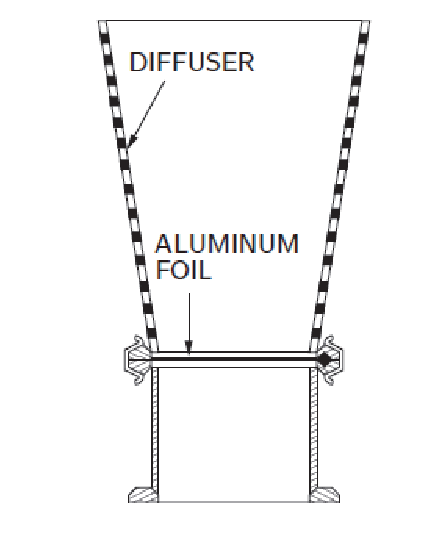
\includegraphics[scale=0.7]{chpt7/figs/fig7.21.eps}
	\caption{混合III低温容器的爆破盘(带扩散器)布置方式。}
\end{figure}

\textbf{混合III低温容器的“爆破盘”和扩散器}

如第3章所述,混合磁体的主要故障是由内插磁体烧坏引发的;
如果应对内插磁体烧坏事件---应急事件,混合III SCM设计了快速放电(这种快速放电模式将在第8章进一步讨论)。

这种快速放电的一个重要后果是低温恒温器压力迅速升高。
混合III低温恒温器配有“爆破盘”,可将低温恒温器的压力增加限制到1 atm;
将40 $\mu$m厚的铝箔盘(有效直径70 mm)安装在真空接头中(图7.21)。
当在低温恒温器的过压超过1 atm时,箔片破裂,从而减轻低温恒温器的压力。
如图所示,扩散器安装在爆破盘出口处,以使出现的蒸汽的出口压力损失最小化。

\subsubsection{问题7.7之解}
a) 第1步中的主要耗散源是磁滞损耗。 
我们计算了Nb3Sn线圈的$E_{hy1}$和NbTi线圈的$E_{hy2}$。
 虽然存在传输电流(高达800 A),但我们对各线圈使用方程7.28c($H_m\gg H_p$):
\begin{align*}% page451 7.28c和S7.1
e_{hy}\simeq\frac{8}{3}\mu_oH_pH_m \tag{7.28c}
\end{align*}
其中,$B_p=\mu_0 H_p$,$B_m=\mu_0 H_m$:
\begin{align*}
e_{hy}=\simeq\frac{8B_pB_m}{3\mu_o} \tag{S7.1}
\end{align*}
Nb3Sn线圈的$E_{hy1}$和NbTi线圈的$E_{hy2}$的总能量耗散为:
\begin{align*}% page451 S7.1a
E_{hy1}=\mathcal{V}_{f1}e_{hy} \tag{S7.1a}
\end{align*}
\begin{align*}% page451 S7.1b
E_{hy2}=\mathcal{V}_{f2}e_{hy} \tag{S71.b}
\end{align*}
其中,$\mathcal{V}_{f1},\mathcal{V}_{f2}$分别是Nb3Sn线圈和NbTi线圈的细丝总体积,分别是:
\begin{align*}% page451 S7.2a
\nu_{f1}=N_{f1}\ell_{cd1}\left(\frac{\pi d_{f1}^{2}}{4}\right) \tag{S7.2a}
\end{align*}
\begin{align*}% page451 S7.2b
\nu_{f2}=N_{f2}\ell_{cd2}\left(\frac{\pi d_{f2}^{2}}{4}\right) \tag{S7.2b}
\end{align*}
式中,$N_f,\ell_{cd},d_f$分别是导体中细丝总数、总导体长度和细丝直径。下标1和2分别表示Nb3Sn和NbTi线圈。

将表7.10中合适的值代入S7.2a和S7.2b,加上$B_{m1}$=4.3 T以及$B_{m2}$=1.8 T,我们得到:
\begin{align*}% page451 S7.3a
E_{hy1}&=(1000)(1700\ \mathrm{m})\frac{\pi(50\times 10^{-6}\ \mathrm{m})^2}{4} 
\times\left(\frac{8}{3}\right)\times\frac{(0.16\ \mathrm{T})(4.3\ \mathrm{T})}{(4\pi\times 10^{-7}\ \mathrm{H/m})} \\
&=(3.3\times 10^{-3}\ \mathrm{m^3})(1.46\times 10^6\ \mathrm{J/m^3})\\ \tag{S7.3a}
&\simeq 4.9\ \mathrm{kJ}
\end{align*}
\begin{align*}% page451 S7.3b
E_{hy1}&=(2500)(8100\ \mathrm{m})\frac{\pi(75\times 10^{-6}\ \mathrm{m})^2}{4} 
\times\left(\frac{8}{3}\right)\times\frac{(0.14\ \mathrm{T})(1.8\ \mathrm{T})}{(4\pi\times 10^{-7}\ \mathrm{H/m})} \\
&=(89.4\times 10^{-3}\ \mathrm{m^3})(0.53\times 10^6\ \mathrm{J/m^3})\\ \tag{S7.3b}
&\simeq 48\ \mathrm{kJ}
\end{align*}

进入液体的总磁滞损耗$\sim$53 kJ。

250 L液氦在1.70 K下的质量为37 kg。
1 atm下,1.70 K氦的焓为1280 J/kg,1.80 K氦的焓为1530 J/kg(附录II),焓变250 J/kg。
总质量为37 kg时,工质池温从1.70 K升至1.80 K需要的净能量输入约10 kJ;
在1200 s的时间内,20 W的制冷机可从液体中移除约25 kJ能量:而液体从1.7 K升至1.8 K需要约35 kJ的总能量。
所以,我们计算的耗散能量$\sim$53 kJ大约高估了两倍。
考虑到上述分析本就是为了给出一个粗略数据,这个结果不算太差;它确切的表明。磁滞损耗是耗散的主要来源。

b) NbTi线圈的总磁滞能量耗散$\sim$30 kJ(如上修正,为$\sim$48 kJ的5/8)在
1200 s内释放,即整体磁滞耗散率为$\sim$25 W。
对线圈2中32个双饼中的每一个,耗散率约0.8 W。
在最保守的条件下,每个双饼的总通道横截面为$\sim 4\ \mathrm{cm^2}$(最内直径658 mm对应的周长乘上通道高度0.5 mm的40\%)---
注意,1 mm高的通道是由两个饼共用的。所以,等效热通量为$\sim 0.2\ \mathrm{W/cm^2}$。
由于热量在径向可以向内也可向外流动,因此通道长度的适当值是o.d和i.d.之间差值的四分之一或$\sim$6 cm。

因为耗散发生在整个通道长度内,可以使用4.6c,即:
\begin{align*}% page452 4.6c
X(T_b)=\frac{q_{c}^{3.4}}{4.4}L \tag{4.6c}
\end{align*}
由图4.9,我们有$X(T_b$=1.8 K)=350。代入$L$=6 cm,在4.6c中解出$q_c=5.1\ \mathrm{W/cm^2}$,
它比最低要求值$\sim 0.2\ \mathrm{W/cm^2}$大很多。
也就是说,通道完全可以在从0到800 A的充电时间将磁滞损耗带走。
实际的运行也验证了这个结论。

c) 在快速变化的场下,最重要的损耗是耦合损耗和涡流损耗。
这里我们仅考虑耦合损耗,因为在没有涡流的情况下,它自身也足以令导体--氦单位体积升温至$T_\lambda$。

我们首先计算NbTi导体的耦合时间常数:
\begin{align*}% 7.6
\tau_{cp}=\frac{\mu_o\ell_{p}^{2}}{8\pi^2\rho_{ef}} \tag{7.6}
\end{align*}

对NbTi复合导体,方程7.7b给出的$\rho_{ef}$常被使用。
以铜-超导体比率$\gamma_{c/s}$表示的$\rho_{ef}$为:
\begin{align*}% page452 7.7b和S7.4
\rho_{ef}&=\frac{1+\lambda_f}{1-\lambda_f}\rho_{m} \\
&=\frac{\gamma_{c/s}+2}{\gamma_{c/s}}\rho_{m} \tag{S7.4}
\end{align*}

由$\gamma_{c/s}=2.2$(从表7.10中给出的导体参数得到),并代入合适的值,由7.6,我们有$\tau_{cp}\simeq 0.17\simeq 0.2$ s,和内插放电的$\tau_m$=0.3 s有可比性。

应用表7.8中的方程7.36和7.39a,将因子$1/2$(仅放电)和$H_m=B_m/\mu_0$以及$D_{mf}=b$代入7.36,有:
\begin{align*}% page453 S7.5a和7.5b
e_{cp}&=\frac{1}{2}\times 2\frac{B_{m}^{2}}{\mu_o}\left[1+\frac{1}{4}\left(\frac{\pi b}{\ell_{p}}\right)^2\right]\times\frac{2\tau_{cp}}{\tau_m}\left[1-\frac{2\tau_{cp}}{\tau_m}\tanh\left(\frac{\tau_m}{2\tau_{cp}}\right)\right] \\
&=\frac{2B_{m}^{2}\tau_{cp}}{\mu_o\tau_m}\left[1+\frac{1}{4}\left(\frac{\pi b}{\ell_{p}}\right)^2\right]\left[1-\frac{2\tau_{cp}}{\tau_m}\tanh\left(\frac{\tau_m}{2\tau_{cp}}\right)\right] \tag{S7.5b}
\end{align*}
代入合适的值,有:
\begin{align*}% page453第二个大公式
e_{cp}\simeq&\frac{2(1\ \mathrm{T})^2(0.2\ \mathrm{s})}{(4\pi\times 10^{-7}\ \mathrm{H/m})(0.3\ \mathrm{s})}\times \\
&\{1+\frac{1}{4}\left[\frac{\pi(2.6\times 10^{-3}\ \mathrm{m})}{0.1\ \mathrm{m}}\right]^2\}\{1-\frac{2(0.2\ \mathrm{s})}{(0.3\ \mathrm{s})}\tanh\left[\frac{(0.3\ \mathrm{s})}{2(0.2\ \mathrm{s})}\right]\}  \\
\simeq&(1.05\times 10^6\ \mathrm{J/m^3})(1)(0.15)\sim 0.16\times 10^6\ \mathrm{J/m^3}
\end{align*}

考虑单位长度(1 cm)的导体。
由于其横截面为(0.92 cm)$\times$(0.26 cm)=0.24 $\mathrm{cm^2}$,
故导体体积$\mathcal{V}_{cd}=0.24\ \mathrm{cm^3}$。
在该导体长度上,氦在2.6 mm宽的导体上占据0.4 cm长度(40\%填充)和0.5 mm通道深度(1 mm深
的通道由顶部和底部饼导体共享)。
因此,对于单位导体长度,氦占据的体积$\mathcal{V}_{he}=5.2\times 10^{-3}\ \mathrm{cm^3}$。
所以,单位导体长度上的总耗散能量$E_{cp}$将由下式给出:
\begin{align*}% page453 S7.9
E_{cp}=e_{cp}\mathcal{V}_{cd}
\sim(0.16\ \mathrm{J/cm^3})\times(0.24\ \mathrm{cm^3})\sim 38\ \mathrm{mJ} \tag{S7.9}
\end{align*}

将单位导体(和响应的液氦)cong 1.8 K加热至$T_\lambda$所需总热能$\Delta E_{th}$:
\begin{align*}% page453 S7.10
E_{th}[h_{cu}(T_\lambda)-h_{cu}(1.8\ \mathrm{K})]\mathcal{V}_{cd}+[h_{he}(T_\lambda)-h_{he}(1.8\ \mathrm{K})]\mathcal{V}_{cd} \tag{S7.10}
\end{align*}
代入$\Delta h_{cu}\simeq 0.1\ \mathrm{mJ/cm^3}$和$\Delta h_{he}\simeq 290\ \mathrm{mJ/cm^3}$,有:
\begin{align*}% page453 S7.11
E_{th}=(0.1\ \mathrm{mJ/cm^3})(0.24\ \mathrm{cm^3})+(290\ \mathrm{mJ/cm^3})(5.2\times 10^{-3}\ \mathrm{cm^3}) \\\tag{S7.11}
\sim 2\ \mathrm{mJ}
\end{align*}
因为$E_{cp}\gg E_{th}$,围绕单位导体的所有液氦都将被加热超过$T_\lambda$,使导体不能失超恢复。



\subsection{讨论7.7:混合III NbTi线圈中的接头耗散}
混合III磁体的NbTi线圈由32个双饼组成,每一个都是有两种等级的9.2 mm宽NbTi复合带绕成的。
各单饼中,高场(HF)级导体和低场(LF)级导体在$r$=378 mm处以“握手”形式接头;
各双饼中,有两个类似的接头。
此外,各双饼的$r$=455 mm处还有另一个接头,用以连接两个相邻的双饼。
混合III磁体在$r$=378 mm处总共有64个接头,在$r$=455 mm处有32个接头。
保守估计,我们选择50Sn-50Pb(表7.1)中$R_{ct}$的较高值:
$R_{ct}$在1 T时为$3.3\times 1-^{-12}\ \mathrm{\Omega m}$,在3 T时为$4.1\times 1-^{-12}\ \mathrm{\Omega m}$。

\textbf{A. 接头电阻}

应用方程7.9b,计算$r$=378 mm处的电阻$R_{sp1}$:
\begin{align*}% page454 7.9b两个
R_{sp}=&\frac{R_{ct}}{A_{ct}}\\\tag{7.9b}
R_{sp1}=&\frac{R_{ct}}{a\ell_{sp1}}
\end{align*}
在上面的方程中,$a\ell_{sp1}=A_{ct}$,$a$是导体宽度,$\ell_{sp}$是接头搭接长度,为$\pi r_{sp1}/2$,
其中$r_{sp1}$为接头位置的绕组半径。
代入$R_{ct}=4.1\times 10^{-12}\ \mathrm{\Omega m^2},a=9.2\times 10^{-3}$ m,$\pi/2$=1.57,,$r_{sp1}$=0.378 m,有:
\begin{align*}% page454 第三个
R_{sp1}=\frac{(4.1\times 10^{-12}\ \mathrm{\Omega m^2})}{(9.2\times 10^{-3}\ \mathrm{m})(1.57\times 0.378\ \mathrm{m})}=0.75\ \mathrm{n\Omega}
\end{align*}
类似的,在$r$=455 mm处:
\begin{align*}% page454第四个
R_{sp2}=\frac{(3.3\times 10^{-12}\ \mathrm{\Omega m^2})}{(9.2\times 10^{-3}\ \mathrm{m})(1.57\times 0.455\ \mathrm{m})}=0.50\ \mathrm{n\Omega}
\end{align*}
总的接头电阻为:
\begin{align*}% page454 第五个
R_{sp}=64R_{sp1}+32R_{sp2}=48\ \mathrm{n\Omega}+16\ \mathrm{n\Omega}=64\ \mathrm{n\Omega}
\end{align*}

\textbf{B. 总接头损耗}

在$I_{op}=$2100 A时的总接头损耗$P_{sp}$为:
\begin{align*}% page454 S8.5
P_{sp}=R_{sp}I_{op}^{2}=(64\times 10^{-9}\ \mathrm{\Omega})(2.1\times 10^3\ \mathrm{A})=0.28\ \mathrm{W}\tag{S8.5}
\end{align*}

在2100 A时不足1 W的接头损耗与混合III运行获得的数据一致。
系统无传输电流时,系统可达到的最低温度为1.65 K;在2100 A时也是如此。
也就是说,与1.65 K时的静态制冷负荷相比,接头损耗可忽略不计。


\subsection{讨论7.8:持续模式运行\&“指数”}

\begin{figure}[htbp]
	\centering
	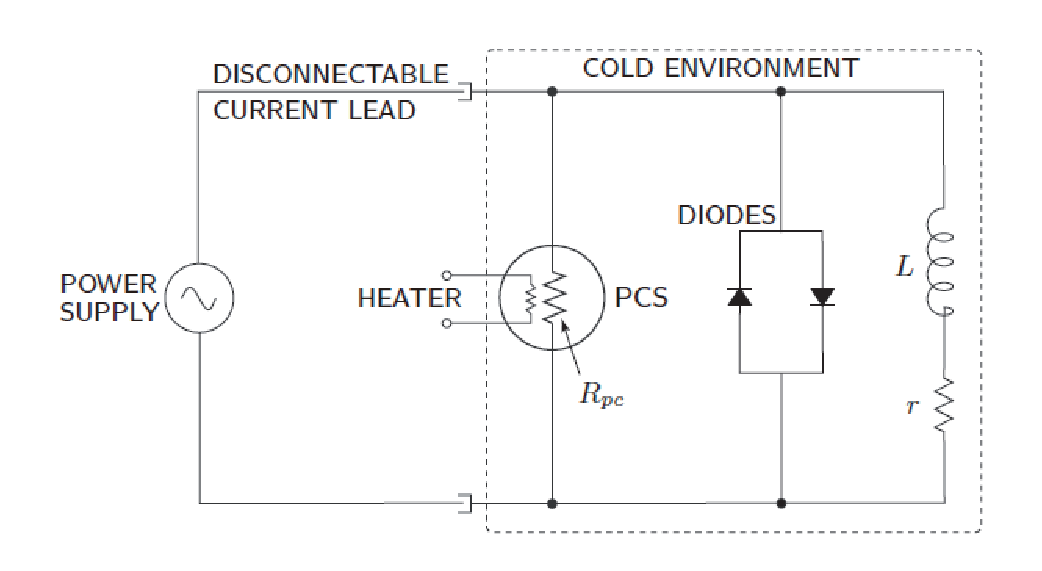
\includegraphics[scale=0.7]{chpt7/figs/fig7.22.eps}
	\caption{Basic circuit diagram for a persistent-mode superconducting magnet。}
\end{figure}




\begin{equation}% page457 6.25b
E_s=E_c\left(\frac{J_s}{J_c}\right)^n
\end{equation}
\begin{equation}% 7.44
V_n=E\ell_{mx}=E_c\left(\frac{I_{op}}{I_c}\right)^n\ell_{mx}
\end{equation}
\begin{equation}% 7.45
\frac{dI_{op}}{dt}=-\frac{V_n}{L_m}=-\frac{E_c}{L_m}\left(\frac{I_{op}}{I_c}\right)^n\ell_{mx}
\end{equation}
\begin{equation}% 7.46两个
\frac{dH}{dt}=-\left(\frac{\Delta H}{\tau_p}\right)\propto-\frac{E_c}{L_m}\left(\frac{I_{op}}{I_c}\right)^n\ell_{mx}
\left(\frac{\Delta H}{H_o\tau_p}\right)=\frac{E_c}{L_m I_{op}}\left(\frac{I_{op}}{I_c}\right)^n\ell_{mx}
\end{equation}
\begin{equation}%  7.47a
\frac{I_{op}}{I_c}\leq\left[\frac{L_mI_{op}}{E_c\ell_{mx}}\left(\frac{\Delta H}{H_o\tau_p}\right)\right]^{1/n}
\end{equation}
\begin{equation}% 7.47b
\frac{I_{op}}{I_c}=\left[\frac{(300\ \mathrm{A})(100\ \mathrm{H})}{(10^{-7}\ \mathrm{V/cm})(10^5\ \mathrm{cm})}(2.78\times 10^{-12}\ \mathrm{/s})\right]^{1/n}
\end{equation}
\begin{equation}% 7.48
n=\frac{\ln(V_2/V_1)}{\ln(I_2/I_1)}
\end{equation}



\begin{figure}[htbp]
	\centering
	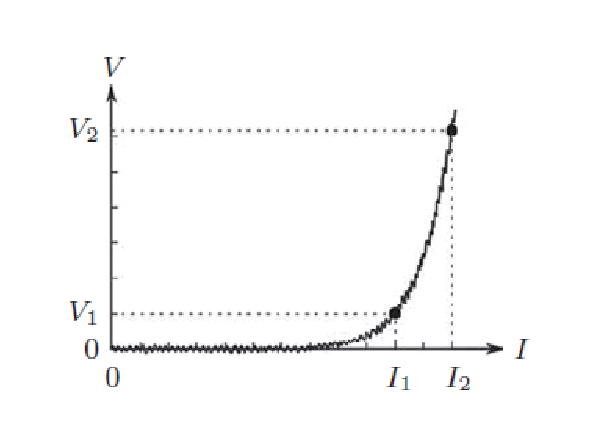
\includegraphics[scale=0.7]{chpt7/figs/fig7.23.eps}
	\caption{Typical V vs. I trace from which to determine an index number.。}
\end{figure}


